\documentclass[11pt]{ppges} 
\usepackage[brazilian]{babel} 
\usepackage[pt-BR]{datetime2}
\usepackage{enumerate}
\usepackage{amsthm}
\usepackage{tikz}
\usepackage{silence}
\usetikzlibrary{arrows.meta,positioning}
\bibliographystyle{apalike}

\newtheorem{lemma}{Lema}
\newtheorem{corollary}{Corolário}
\makeatletter
\providecommand*{\toclevel@algorithm}{0}
\makeatother
\WarningFilter{latex}{Text page}
\hfuzz=30pt
\hbadness=10000
\emergencystretch=2em

\newcommand{\warn}[1]{{\color{red} {#1}}}
\newcommand{\warnadv}[2]{
{\color{red} {#1}} {\color{blue} \begin{quote}\emph{\small{{#2}}}\end{quote}}}

\newcommand{\field}[1]{{\sc {#1}}}
 
\graphicspath{{./figures/}}

\newcommand\dtitle{Biobunker como Combustível de Transição no Transporte Marítimo: Viabilidade e Estratégias para a Descarbonização no Brasil}

\newcommand\dauthor{Maria Izabel Barreto Ogasawara}
\newcommand\dadvisor{Nival Nunes de Almeida}
\newcommand\djury{
	\HRule \\ Presidente, Prof. Nival Nunes de Almeida, D.Sc. (orientador) \\[0.8cm]
	\HRule \\ Membro 1, D.Sc. \\[0.8cm]
	\HRule \\ Membro 2, D.Sc. \\[2.5cm]
}

\makeglossaries

\newacronym{IMO}{IMO}{International Maritime Organization}
\newacronym{GEE}{GEE}{Gases de Efeito Estufa}
\newacronym{MLP}{MLP}{Multi-Level Perspective}
\newacronym{EUETS}{EU ETS}{European Union Emissions Trading System}
\newacronym{ICCT}{ICCT}{International Council on Clean Transportation}
\newacronym{IEA}{IEA}{International Energy Agency}
\newacronym{DNV}{DNV}{Det Norske Veritas}
\newacronym{LNG}{LNG}{Liquefied Natural Gas}
\newacronym{CCS}{CCS}{Carbon Capture and Storage}
\newacronym{MARPOL}{MARPOL}{International Convention for the Prevention of Pollution from Ships}
\newacronym{ECA}{ECA}{Emission Control Area}
\newacronym{CBIO}{CBIO}{Crédito de Descarbonização}
\newacronym{ACV}{ACV}{Avaliação de Ciclo de Vida}
\newacronym{TEA}{TEA}{Techno-Economic Assessment}
\newacronym{PECA}{PECA}{População, Exposição, Comparação, Avaliação}
\newacronym{LCOS}{LCOS}{Levelized Cost of Service}
\newacronym{ILUC}{ILUC}{Indirect Land Use Change}
\newacronym{SOx}{SOx}{Óxidos de Enxofre}
\newacronym{ISO}{ISO}{International Organization for Standardization}
\newacronym{WTW}{WTW}{Well-to-Wake}
\newacronym{WTT}{WTT}{Well-to-Tank}
\newacronym{TTW}{TTW}{Tank-to-Wake}
\newacronym{UCO}{UCO}{Used Cooking Oil}
\newacronym{TCO}{TCO}{Technical Corn Oil}
\newacronym{B24}{B24}{Mistura com 24\% de Biodiesel}
\newacronym{B20}{B20}{Mistura com 20\% de Biodiesel}
\newacronym{B15}{B15}{Mistura com 15\% de Biodiesel}

\begin{document}

\hypersetup{pageanchor=false}
\pagenumbering{gobble}

\dcover

\dsignatures

\dlibrary{ficha.pdf}
	
\ddedicatory{
	\raggedleft \normalsize Seção reservada à dedicatória.
}

\dacknowledgment{
	Seção reservada a agradecimentos.
	
	Agradece-se à CAPES pelo financiamento parcial do projeto.
}

\dresumo{Esta dissertação analisa a viabilidade técnica, econômica e ambiental do biobunker, definido como a mistura de biodiesel com bunker fuel, como combustível de transição no transporte marítimo. O estudo insere-se no contexto das metas de descarbonização estabelecidas pela Organização Marítima Internacional para 2030 e da necessidade de avaliar alternativas capazes de reduzir emissões no curto e médio prazo, enquanto combustíveis de emissão zero amadurecem tecnologicamente. A análise baseia-se em simulações com dados reais de operação de navios, em estimativas de impactos ambientais derivadas de estudos de Avaliação de Ciclo de Vida (ACV) disponíveis na literatura e na avaliação de custos e restrições logísticas associadas ao uso do biobunker. Adicionalmente, o trabalho examina o papel do arcabouço institucional e das políticas públicas brasileiras na adoção desse combustível pelo setor marítimo. Ao investigar o biobunker como alternativa intermediária na transição energética, a dissertação contribui para a compreensão de suas possibilidades e limitações no contexto do transporte marítimo brasileiro.}{bunker fuel, biodiesel, biobunker, descarbonização, transporte marítimo}

\dabstract{This dissertation analyzes the technical, economic, and environmental feasibility of biobunker, defined as a blend of biodiesel and bunker fuel, as a transitional fuel in maritime transport. The study is situated within the context of the decarbonization targets established by the International Maritime Organization for 2030 and the need to assess alternatives capable of reducing emissions in the short and medium term while zero-emission fuels continue to mature technologically. The analysis is based on simulations conducted using real ship operational data, the use of environmental impact estimates derived from Life Cycle Assessment (LCA) studies available in the literature, and the evaluation of costs and logistical constraints associated with biobunker deployment. In addition, the dissertation examines the role of Brazil's institutional framework and public policies in shaping the adoption of this fuel within the maritime sector. By investigating biobunker as an intermediate option in the energy transition, the dissertation contributes to understanding its potential and limitations in the context of Brazilian maritime transport.}{bunker fuel, biodiesel, biobunker, decarbonization, maritime transport}

\dtables
\hypersetup{pageanchor=true}


\pagenumbering{arabic}
\justifying

\chapter{Introdução}
\label{chap_introducao}

O transporte marítimo responde por mais de 80\% do comércio global de mercadorias, configurando-se como o meio mais eficiente para o transporte de cargas em grande escala \citep{unctad_transport_2025}. No entanto, o transporte marítimo internacional também contribui de forma relevante para os problemas ambientais globais, uma vez que os combustíveis utilizados nos navios mercantes são predominantemente \emph{bunker fuel}, combustível fóssil derivado de hidrocarbonetos que libera gases nocivos na atmosfera, como óxidos de enxofre ($SO_x$) e dióxido de carbono ($CO_2$) \citep{international_maritime_organization_fourth_2020,van_global_2019}.

Em razão da importância estratégica que exerce nas relações comerciais e, portanto, na economia mundial, o transporte marítimo integra os debates sobre redução de emissões de \gls{GEE} promovidos por organismos multilaterais, entre eles a \gls{IMO}, responsável pela regulação do setor \citep{international_maritime_organization_fourth_2020,imo2023strategy}. O setor enfrenta, assim, desafios significativos para atingir as metas de redução da intensidade de carbono, especialmente diante das restrições impostas pela \gls{IMO} 2020. Essas metas estabelecem objetivos para 2030 e 2050 \citep{imo_imo_2020,imo2023strategy}, conforme descrito a seguir:

\begin{itemize}
  \item Metas para 2030: reduzir a intensidade de carbono em 40\% em relação aos níveis de 2008, promovendo maior eficiência energética e o uso de combustíveis de baixa emissão.
  \item Metas para 2050: reduzir as emissões absolutas em 50\% em comparação a 2008 e alcançar a neutralidade de carbono por meio de combustíveis de emissão zero e tecnologias limpas.
\end{itemize}

As opções para o atingimento do objetivo de descarbonização incluem intervenções tecnológicas e inovações voltadas à melhoria da eficiência energética e operacional dos meios marítimos. Contudo, para alcançar as metas definidas pela \gls{IMO}, torna-se necessária a substituição dos combustíveis fósseis por fontes alternativas de energia \citep{imo2023strategy,international_council_on_clean_transportation_potential_2021}.

O hidrogênio verde é apontado na literatura como referência relevante de longo prazo para o atingimento das metas de descarbonização do transporte marítimo até 2050, por apresentar potencial de emissão zero de carbono quando produzido a partir de fontes renováveis. Quando utilizado em células de combustível, elimina as emissões de $CO_2$, enxofre ($SO_x$) e particulados. No entanto, sua adoção enfrenta desafios no curto prazo, tais como:

\begin{itemize}
  \item Infraestrutura: requer o desenvolvimento de sistemas para produção, armazenamento e abastecimento, envolvendo investimentos elevados e prazos extensos \citep{lin_alternative_2023};
  \item Custo: apresenta custo elevado atualmente, em razão do alto custo de produção por eletrólise \citep{hansson_potential_2020};
  \item Tecnologia dos navios: exige novos motores ou células de combustível, além de tanques especializados para armazenamento, o que dificulta sua implementação em larga escala até 2030 \citep{tornatore_ammonia_2022}.
\end{itemize}


Enquanto essa alternativa não for viável, o setor marítimo precisa reduzir emissões de \gls{GEE} em consonância com metas internacionais, mantendo parâmetros operacionais e custos compatíveis com sua função no comércio global. Nesse intervalo, o biobunker, definido como a mistura de biodiesel (biocombustível produzido a partir de fontes renováveis, como óleos vegetais e gorduras animais, que apresenta caráter biodegradável \citep{paulauskiene_alternative_2019}) com \emph{bunker fuel}, surge na literatura como combustível de transição com potencial para reduzir parcialmente as emissões antes da adoção mais ampla de tecnologias de emissão zero \citep{irena_pathway_2021,roux_review_2024}.

Em contextos específicos, essa alternativa pode reduzir emissões de $CO_2$, $SO_x$ e particulados, ser utilizada em motores atuais com pouca ou nenhuma modificação e, quando produzida a partir de resíduos, contribuir para a economia circular e para a redução de impactos ambientais \citep{bilgili_comparative_2021,altarazi_effects_2022,emaf_towards_2013}.

Embora não seja capaz de atingir a neutralidade de carbono proposta para 2050, o biobunker pode contribuir para a redução de emissões no curto prazo em razão da infraestrutura existente, da relativa facilidade de adoção e, em alguns contextos, da menor barreira de implementação em comparação com rotas mais disruptivas \citep{international_council_on_clean_transportation_potential_2021,altarazi_effects_2022,petzold_operation_2011}. Além disso, pode representar alternativa mais acessível para o atendimento das metas intermediárias da \gls{IMO} até 2030, especialmente em países com abundância de biomassa, como o Brasil \citep{carvalho_biofuels_2021}.

Embora as metas de descarbonização do transporte marítimo sejam definidas em âmbito global pela \gls{IMO}, a adoção de combustíveis alternativos no curto prazo é condicionada por instrumentos regulatórios regionais e por exigências de mercados específicos. Em particular, rotas internacionais que conectam países produtores de combustíveis, como o Brasil, a grandes mercados consumidores, como a União Europeia, estão sujeitas a pressões regulatórias externas que influenciam as decisões operacionais dos armadores, independentemente da bandeira do navio ou do local de abastecimento do combustível \citep{eu_reg_2023_957,eu_reg_2023_1805}.

Nesse contexto, a análise do biobunker como combustível de transição no transporte marítimo internacional operando a partir do Brasil adquire relevância não apenas por suas características técnicas e ambientais, mas também por sua potencial adequação a exigências regulatórias internacionais que afetam a competitividade das rotas marítimas \citep{carvalho_biofuels_2021,eu_reg_2023_957}.

Por essa razão, este estudo adota como referência um cenário de navegação internacional entre portos brasileiros e europeus. A escolha da rota Brasil–Europa fundamenta-se em três fatores principais. Em primeiro lugar, a União Europeia se destaca como o principal polo regulatório global no processo de descarbonização do transporte marítimo, com a implementação de instrumentos como o \gls{EUETS} e o regulamento FuelEU Maritime, que introduzem custos diretos associados às emissões de dióxido de carbono e metas progressivas de redução da intensidade de carbono dos combustíveis \citep{eu_reg_2023_957,eu_reg_2023_1805}.

Em segundo lugar, essa rota tem relevância econômica significativa, uma vez que a União Europeia figura entre os principais parceiros comerciais do Brasil, representando parcela expressiva do fluxo de comércio exterior e, consequentemente, do tráfego marítimo internacional. Por fim, a aplicação extraterritorial desses instrumentos regulatórios, que incidem sobre navios que escalam portos europeus independentemente do local de abastecimento, torna essa rota particularmente adequada para analisar, de forma integrada, os efeitos econômicos e ambientais associados à adoção de combustíveis de menor intensidade de carbono \citep{carvalho_biofuels_2021,eu_reg_2023_957}.

Desse modo, o recorte geográfico adotado não apenas reflete a relevância empírica da rota, mas amplia também a capacidade explicativa do modelo ao incorporar explicitamente sinais regulatórios que influenciam a viabilidade das alternativas energéticas no curto prazo.

No Brasil, a aplicação do biobunker carece de estudos integrados que avaliem seu desempenho sob premissas técnicas explícitas de compatibilidade operacional, articulando custos, impactos ambientais e condicionantes regulatórios com base em parâmetros operacionais representativos. Também não há consenso sobre sua inserção no setor a partir de instrumentos institucionais e regulatórios \citep{carvalho_biofuels_2021}. Essa lacuna orienta a presente pesquisa.

Diante dessas premissas, estabelece-se a seguinte pergunta de pesquisa: sob premissas técnicas de compatibilidade operacional, o biobunker pode ser considerado alternativa econômico-ambientalmente viável para apoiar a transição energética do transporte marítimo internacional operando a partir do Brasil, considerando as metas de descarbonização da \gls{IMO} até 2030 e os condicionantes regulatórios associados a rotas internacionais?

Para responder a essa pergunta, o objetivo geral é desenvolver um modelo determinístico de simulação comparativa \emph{in silico}, aplicado a uma rota representativa do transporte marítimo internacional operando a partir do Brasil, que permita avaliar a viabilidade econômico-ambiental do biobunker sob premissas técnicas de compatibilidade operacional. Essa avaliação considera os efeitos da fração de mistura e da rota de produção do biodiesel sobre o consumo requerido, as emissões no escopo \emph{well-to-wake}, o custo total por viagem e o custo marginal de abatimento de carbono, à luz das metas de descarbonização da \gls{IMO} até 2030 e dos condicionantes regulatórios associados à rota analisada.

Em termos argumentativos, a dissertação se organiza em torno de três contribuições principais. A primeira consiste em propor um arcabouço integrado para comparar cenários de biobunker a partir da articulação entre desempenho operacional agregado, emissões no escopo \emph{well-to-wake}, custo total por viagem e custo marginal de abatimento de carbono. A segunda consiste em aplicar esse arcabouço a uma rota representativa do transporte marítimo internacional operando a partir do Brasil, incorporando explicitamente a heterogeneidade entre rotas de produção do biodiesel. A terceira consiste em interpretar os resultados à luz do ambiente regulatório europeu incidente sobre rotas Brasil--Europa, distinguindo entre custo explícito de \emph{compliance} e parâmetro de referência para avaliação da atratividade econômico-ambiental.

Com base nessa estrutura, a dissertação trata a compatibilidade técnica do uso de misturas como premissa operacional delimitada no modelo e concentra sua verificação empírica na existência, ou não, de combinações entre fração de mistura e rota de produção do biodiesel que satisfaçam simultaneamente critérios ambientais e econômico-regulatórios. Essa operacionalização é formalizada no capítulo de método por meio de uma hipótese de existência de cenários viáveis no domínio analisado.

Além desta introdução, a dissertação está organizada em mais quatro capítulos. O Capítulo~\ref{chap_referencial} apresenta a revisão da literatura e o referencial teórico que sustentam a análise. O Capítulo~\ref{chap_metodo} descreve o método, as premissas de modelagem e os critérios de avaliação adotados. O Capítulo~\ref{chap_resultados} expõe os resultados parciais da simulação e sua discussão. Por fim, o Capítulo~\ref{chap_conclusao} reúne as considerações parciais da pesquisa e os encaminhamentos para as etapas seguintes do trabalho.


\chapter{Revisão da Literatura}
\label{chap_referencial}

Este capítulo está estruturado em duas partes: o referencial teórico, que apresenta os conceitos fundamentais para a compreensão do tema, e os trabalhos relacionados, que discutem as principais contribuições acadêmicas e aplicações recentes, articulando abordagens da literatura, comparações entre rotas tecnológicas e lacunas de pesquisa.

\section{Referencial teórico}
O referencial teórico desta dissertação está estruturado em três vertentes complementares: sustentabilidade e metas globais, tecnologias de combustíveis alternativos e adaptação do setor marítimo brasileiro. Em conjunto, essas dimensões fornecem a base conceitual necessária para compreender os desafios e as possibilidades da transição energética no transporte marítimo.

\subsection{Sustentabilidade e Metas Globais}
A discussão sobre a transformação do transporte marítimo está associada ao conceito de sustentabilidade e às agendas globais voltadas à mitigação das mudanças climáticas. A literatura mobiliza referenciais normativos e interpretativos que ajudam a compreender por que a transição energética do setor se tornou tema central no debate internacional.

O conceito de sustentabilidade proposto por \citet{elkington_cannibals_1998}, por meio do \emph{Triple Bottom Line}, constitui um referencial central. Ao articular os pilares econômico, ambiental e social, essa abordagem amplia a análise do desempenho do setor marítimo, indicando que decisões relacionadas a custos operacionais, eficiência energética e escolha de combustíveis não podem ser avaliadas isoladamente. Ao contrário, devem considerar, simultaneamente, os impactos ambientais associados às emissões atmosféricas e as implicações sociais decorrentes da atividade marítima. Esse enquadramento teórico legitima abordagens multicritério na avaliação de alternativas tecnológicas e energéticas para o setor.

As metas ambientais estabelecidas pela \gls{IMO}, particularmente aquelas relacionadas à redução do teor de enxofre nos combustíveis marítimos e à descarbonização progressiva até 2050, refletem esse alinhamento com agendas globais de sustentabilidade. Conforme discutido por \citet{van_global_2019}, as regulações da \gls{IMO} impõem limites rigorosos ao teor de enxofre, inicialmente em áreas de controle de emissões e, posteriormente, de forma global, o que desencadeia mudanças significativas nos processos de refino e na composição do \emph{mix} de combustíveis utilizados na navegação. Os autores destacam que essas medidas contribuem para reduções mensuráveis nas emissões de poluentes atmosféricos, ainda que gerem desafios adicionais relacionados a custos, investimentos e emissões indiretas de \gls{GEE} no processo de refino.

A literatura também enfatiza que tais esforços regulatórios devem ser compreendidos à luz de limites biofísicos mais amplos. \citet{mukherjee_perspective_2020}, ao discutirem o papel dos biocombustíveis e da \gls{CCS} no setor marítimo, ressaltam a necessidade de manter as atividades humanas dentro de limites ambientais compatíveis com a estabilidade do sistema terrestre. Essa perspectiva reforça a centralidade da redução das emissões de \gls{GEE} como elemento estruturante das estratégias de transição energética no transporte marítimo.

Nessa direção, o conceito de limites planetários, formulado por \citet{rockstrom_safe_2009}, figura entre os principais fundamentos científicos das metas globais de descarbonização. Essa abordagem estabelece fronteiras ecológicas críticas que não devem ser ultrapassadas para garantir a estabilidade e a resiliência do sistema terrestre, incluindo limites diretamente associados às mudanças climáticas e às emissões de \gls{GEE}. Ao reconhecer que o crescimento econômico e as atividades produtivas estão condicionados a restrições biofísicas, esse referencial dá base científica à imposição de metas ambientais rigorosas ao setor marítimo. Políticas de redução de emissões e de controle do uso de combustíveis fósseis no transporte marítimo podem, portanto, ser interpretadas não apenas como escolhas regulatórias, mas como respostas institucionais à necessidade de manter o sistema global de transportes dentro de limites ambientalmente seguros.

A discussão é complementada pela distinção entre sustentabilidade forte e fraca, proposta por \citet{daly_sustainable_2006}. Ao enfatizar que determinados recursos naturais são insubstituíveis, essa abordagem reforça as limitações de estratégias baseadas exclusivamente em compensações ou ganhos marginais de eficiência. No contexto do transporte marítimo, isso implica reconhecer que a transição energética não pode se restringir à redução incremental de emissões, mas deve incorporar escolhas que preservem o capital natural e reduzam a dependência estrutural de combustíveis fósseis.

Paralelamente aos fundamentos normativos da sustentabilidade, a literatura sobre transições sociotécnicas oferece aportes relevantes para compreender como essas transformações podem ocorrer na prática. A \gls{MLP}, desenvolvida por \citet{geels_technological_2002,geels_multi-level_2011}, interpreta as transições tecnológicas como processos evolutivos que envolvem a interação entre regimes estabelecidos, inovações emergentes e pressões externas, como mudanças regulatórias e demandas sociais. Sob essa ótica, a substituição do \emph{bunker fuel} por combustíveis alternativos representa a transformação de um regime sociotécnico consolidado, influenciado por regulações ambientais e dinâmicas de mercado.

\citet{schot_strategic_2008} destacam o papel das chamadas \emph{niches}, espaços protegidos que permitem o desenvolvimento e o amadurecimento de inovações sustentáveis. No setor marítimo, combustíveis alternativos, como os biocombustíveis líquidos, podem ser compreendidos como tecnologias de transição, cuja difusão depende de políticas específicas, experimentação controlada e processos de aprendizado que viabilizem reduções de custo e ganhos de escala. Estudos como o de \citet{international_council_on_clean_transportation_potential_2021} indicam que os biocombustíveis podem desempenhar papel relevante na redução das emissões do transporte marítimo, especialmente no curto e médio prazo, enquanto soluções como o hidrogênio ainda enfrentam limitações tecnológicas e de infraestrutura.

Por fim, a teoria da difusão de inovações, proposta por \citet{rogers_diffusion_2003}, contribui para explicar a adoção gradual dessas alternativas energéticas. A introdução progressiva de misturas de biocombustíveis, como B15 e B20, exemplifica um processo incremental, no qual ajustes técnicos, regulatórios e organizacionais permitem a assimilação das inovações pelo setor. Esse processo evidencia que a transição energética no transporte marítimo tende a ocorrer de forma gradual, condicionada por fatores técnicos, econômicos e institucionais.

\subsection{Instrumentos regulatórios europeus e seus efeitos sobre a descarbonização do transporte marítimo}

Embora esta dissertação tenha como foco o contexto brasileiro, a literatura indica que, no curto e médio prazo, vetores decisivos de mudança no transporte marítimo têm origem em iniciativas regulatórias regionais, com destaque para a União Europeia \citep{psaraftis_comparative_2021,eu_reg_2023_957,eu_reg_2023_1805}. Diferentemente das metas globais da \gls{IMO}, que definem objetivos agregados de longo prazo, os instrumentos europeus introduzem sinais econômicos e obrigações operacionais que afetam as decisões dos armadores, independentemente da bandeira do navio ou do local de abastecimento do combustível.

Nesse quadro, dois instrumentos merecem destaque: a inclusão do transporte marítimo no Sistema Europeu de Comércio de Emissões e a adoção do regulamento \emph{FuelEU Maritime}. Esses mecanismos atuam de forma complementar, ao precificar emissões absolutas de dióxido de carbono e, simultaneamente, impor limites à intensidade de \gls{GEE} dos combustíveis utilizados a bordo.

A inclusão do transporte marítimo no \gls{EUETS} representa mudança estrutural na governança climática do setor. Conforme discutido por \citet{psaraftis_comparative_2021}, mecanismos baseados em mercado têm a capacidade de internalizar externalidades ambientais de forma mais imediata do que metas voluntárias ou instrumentos puramente tecnológicos. A partir de 2024, navios que escalem portos da União Europeia passam a ser obrigados a adquirir permissões de emissão para cobrir parte de suas emissões de $CO_2$, com regime de implementação gradual que atinge 100\% das emissões elegíveis a partir de 2026. Para viagens entre portos europeus e portos de países terceiros, 50\% das emissões associadas ao trajeto são incluídas no sistema.

A literatura destaca que esse mecanismo cria custo direto associado ao uso de combustíveis fósseis convencionais, afetando a competitividade operacional das embarcações. \citet{psaraftis_comparative_2021} demonstram que a precificação do carbono no transporte marítimo tende a influenciar decisões de curto prazo, como velocidade, escolha de rotas e, sobretudo, composição do combustível, uma vez que essas decisões permitem reduzir emissões sem a necessidade imediata de investimentos elevados em novos sistemas de propulsão. Nessa perspectiva, o \gls{EUETS} não prescreve tecnologias específicas, mas incentiva economicamente a adoção de soluções capazes de reduzir emissões reportadas.

De forma complementar, o regulamento \emph{FuelEU Maritime}, em vigor a partir de 2025, estabelece limites progressivamente mais rigorosos para a intensidade de \gls{GEE} da energia utilizada a bordo dos navios que tocam portos da União Europeia. Diferentemente do \gls{EUETS}, que incide sobre emissões absolutas, o \emph{FuelEU Maritime} adota abordagem baseada em ciclo de vida, considerando as emissões \emph{well-to-wake}, ou seja, desde a produção do combustível até sua utilização no navio. Essa distinção é relevante, pois desloca o foco regulatório do controle de emissões locais para a avaliação integrada das cadeias energéticas.

Estudos como os de \citet{ce_delft_assessment_2020} indicam que combustíveis renováveis e de baixo carbono, especialmente combustíveis compatíveis com a infraestrutura existente (do inglês, \emph{drop-in fuels}) obtidos de resíduos, são favorecidos pela abordagem de intensidade de carbono ao longo do ciclo de vida promovida pelo regulamento \emph{FuelEU Maritime}, uma vez que podem ser adotados com a tecnologia existente e contribuem para o cumprimento de metas até 2030 antes que combustíveis de emissão zero, como hidrogênio e amônia, estejam amplamente disponíveis.

A combinação entre \gls{EUETS} e \emph{FuelEU Maritime} cria, portanto, duplo vetor de pressão regulatória: por um lado, penaliza economicamente o uso de combustíveis fósseis intensivos em carbono; por outro, estabelece padrões mínimos de desempenho climático para os combustíveis utilizados. Estudos como o de \citet{ce_delft_fueleu_2021} destacam que esse arranjo institucional tende a favorecer soluções de transição capazes de reduzir emissões de forma imediata, sem exigir transformações estruturais profundas na frota ou na infraestrutura portuária no curto prazo, ao alinhar os incentivos de mercado entre o preço do carbono no \gls{EUETS} e os requisitos de intensidade de carbono do \emph{FuelEU Maritime}.

Nesse contexto, os biocombustíveis líquidos surgem na literatura como alternativa intermediária entre o \emph{bunker fuel} e os combustíveis de emissão zero. Estudos como o de \citet{international_council_on_clean_transportation_potential_2021} mostram que combustíveis líquidos derivados de biomassa, como biodiesel de óleos residuais e diesel renovável, podem ser usados em motores marítimos existentes sem grandes modificações, por serem compatíveis com a infraestrutura existente, e apresentam redução de emissões ao longo do ciclo de vida quando comparados ao \emph{bunker fuel}. Estudos de avaliação de ciclo de vida também confirmam que certas rotas de biocombustíveis podem alcançar reduções significativas de \gls{GEE} em comparação com combustíveis fósseis, embora não sejam suficientes, por si só, para alcançar a neutralidade de carbono no longo prazo.

Do ponto de vista geográfico, um aspecto central desses instrumentos regulatórios europeus é que sua aplicação independe do local de abastecimento do combustível. As obrigações do \gls{EUETS} e do \emph{FuelEU Maritime} são acionadas pela escala do navio em portos da União Europeia, e não pela origem do combustível utilizado. Assim, combustíveis abastecidos em portos fora da UE, incluindo portos brasileiros, são considerados nos mecanismos de conformidade, desde que atendam aos critérios de rastreabilidade e elegibilidade estabelecidos pela regulação europeia.

Essa característica amplia o alcance dos instrumentos europeus para além de suas fronteiras territoriais, criando incentivos indiretos para a oferta de combustíveis marítimos de menor intensidade de carbono em portos extraeuropeus, em razão, por exemplo, do impacto da demanda europeia por biocombustíveis sobre mercados internacionais e cadeias de suprimento de combustíveis. Estudos como o de \citet{emsa_potential_2020} indicam que a demanda e a regulação de biocombustíveis na UE afetam fluxos comerciais globais e incentivos para fornecedores extra-regionais. No entanto, a efetividade desses mecanismos depende da robustez dos sistemas de certificação e da disponibilidade sustentável de matérias-primas, pois essas condições influenciam o desempenho ambiental e de ciclo de vida dos combustíveis \citep{cherubini_life_2011}.

\subsection{Tecnologias de Combustíveis Alternativos}
No plano técnico, a transição energética no transporte marítimo se materializa por meio da substituição progressiva do \emph{bunker fuel} por combustíveis de menor intensidade de carbono. Como esse processo é gradual e condicionado por restrições tecnológicas, econômicas e institucionais, a literatura combina interpretações sobre trajetórias tecnológicas, classificações institucionais das rotas energéticas e evidências sobre desempenho, viabilidade e sustentabilidade.

Nesse sentido, a contribuição clássica de \citet{schumpeter_business_2006} oferece primeiro referencial ao compreender a inovação como processo de \emph{destruição criativa}, no qual novos paradigmas tecnológicos substituem soluções estabelecidas, mesmo quando estas são amplamente difundidas e eficientes em seus próprios termos. Aplicado ao setor marítimo, esse raciocínio permite interpretar o abandono progressivo dos combustíveis fósseis tradicionais como resultado da convergência entre pressões regulatórias, ambientais e econômicas, e não apenas como decisão técnica isolada.

\citet{freeman_economics_1997} aprofundam essa leitura ao enfatizar o papel dos paradigmas tecnológicos e das trajetórias de inovação nos processos de transformação industrial. Sob essa perspectiva, os combustíveis alternativos não competem em condições homogêneas, mas se inserem em diferentes estágios de maturidade tecnológica. Os biocombustíveis, em particular, podem ser interpretados como inovações intermediárias, capazes de reduzir emissões e, simultaneamente, aproveitar parte da infraestrutura existente, criando condições para a futura difusão de soluções mais disruptivas, como o hidrogênio e a amônia. Essa abordagem reforça a ideia de que a transição energética no transporte marítimo ocorre em ondas sucessivas, nas quais tecnologias transitórias e de longo prazo coexistem.

Do ponto de vista técnico e institucional, diversas organizações têm proposto classificações que auxiliam na organização desse campo emergente. Relatórios do \gls{ICCT}, da \gls{IEA} e da \gls{DNV} convergem na identificação de cinco grandes categorias de combustíveis alternativos para o transporte marítimo: biocombustíveis, \emph{e-fuels} (combustíveis sintéticos produzidos a partir de hidrogênio e carbono capturado), gás natural liquefeito (\gls{LNG}), amônia e hidrogênio. Essa taxonomia é relevante porque permite comparar rotas tecnológicas distintas em termos de maturidade, potencial de redução de emissões, compatibilidade com motores existentes e necessidades de infraestrutura. Para a análise desenvolvida nesta dissertação, ela também ajuda a distinguir soluções mais próximas da adoção no curto prazo daquelas cuja difusão depende de transformações mais profundas em sistemas de propulsão, armazenamento e abastecimento.

No caso de combustíveis associados ao horizonte de longo prazo, o hidrogênio verde é apontado como alternativa promissora devido à sua capacidade de eliminar emissões diretas de carbono \citep{ustolin_extensive_2022}. Contudo, a literatura indica que barreiras tecnológicas, custos elevados e desafios de infraestrutura tornam sua adoção inviável no curto prazo, especialmente para grandes embarcações, como navios porta-contêineres. Esse cenário reforça a relevância de soluções intermediárias, capazes de reduzir emissões enquanto tecnologias mais disruptivas amadurecem.

Entre essas alternativas, os biocombustíveis têm recebido atenção especial devido ao seu potencial de aplicação no curto e médio prazo. Estudos indicam que o uso de biodiesel e outros biocombustíveis líquidos pode resultar em reduções significativas das emissões de dióxido de carbono em comparação ao \emph{bunker fuel}, além de apresentar desempenho energético compatível com a operação marítima \citep{kesieme_biofuel_2019,masum_comparing_2023,international_council_on_clean_transportation_potential_2021}. Ademais, há evidências de que motores marítimos podem operar com misturas de biodiesel de até B20 sem a necessidade de modificações estruturais relevantes, o que reduz barreiras técnicas à adoção dessas alternativas \citep{altarazi_effects_2022}.

No âmbito conceitual, o biobunker encontra respaldo na economia circular \citep{emaf_towards_2013}, ao enfatizar o uso de resíduos como matéria-prima e a redução da extração de recursos fósseis. A literatura aponta que o biodiesel produzido a partir de fontes residuais, como óleos de cozinha usados, pode reduzir significativamente emissões de \gls{GEE}, monóxido de carbono, hidrocarbonetos e material particulado, além de manter compatibilidade com motores diesel existentes \citep{lopresto_sustainable_2025}. Entretanto, desafios relacionados à estabilidade do combustível, à logística e à disponibilidade de \emph{feedstock} ainda representam barreiras à sua difusão em larga escala \citep{mohd_noor_biodiesel_2018}.

Apesar do potencial técnico, diversos estudos destacam limitações econômicas e institucionais para a adoção dos combustíveis alternativos. \citet{lindstad_reduction_2021} ressaltam os custos de produção e as incertezas de mercado como fatores críticos, especialmente quando comparados aos combustíveis fósseis convencionais. \citet{mukherjee_techno-economic_2023} argumentam que a efetividade das rotas alternativas de descarbonização no setor marítimo depende, em grande medida, de sua integração com tecnologias de \gls{CCS}, ampliando o impacto climático positivo dessas soluções.

Avanço importante na literatura recente é a combinação de análises técnico-econômicas (\gls{TEA}) com avaliações de ciclo de vida (\gls{ACV}), permitindo análise integrada de custos, emissões e impactos ambientais ao longo de toda a cadeia produtiva dos biocombustíveis. Estudos como os de \citet{tan_biofuel_2021} e \citet{li_techno-economic_2022} demonstram que essa abordagem é fundamental para evitar avaliações parciais, que considerem apenas as emissões na fase de uso e negligenciem impactos associados à produção, transporte e processamento do combustível.

Por fim, a viabilidade dos combustíveis alternativos deve ser analisada à luz da sustentabilidade do \emph{feedstock} e dos possíveis efeitos sistêmicos. \citet{zink_circular_2017} alertam para o risco do \emph{rebound effect}, no qual ganhos de eficiência podem ser parcialmente anulados pelo aumento da demanda energética. Nesse contexto, mecanismos de certificação e políticas públicas desempenham papel central na mitigação desses riscos, ao estabelecer critérios de rastreabilidade, intensidade de carbono e uso sustentável de matérias-primas. Iniciativas como a \emph{Renewable Energy Directive} II e III (RED II/RED III), na União Europeia, e o programa RenovaBio, no Brasil, ilustram a incorporação desses princípios no desenho regulatório.

Ao integrar os referenciais de inovação tecnológica, as classificações institucionais, as métricas de desempenho ambiental e as dimensões regulatórias, delineia-se um quadro consistente para compreender o papel dos combustíveis alternativos na substituição do \emph{bunker fuel}. Esse arcabouço evidencia que a transição energética no transporte marítimo é um processo multidimensional, no qual fatores técnicos, econômicos, ambientais e institucionais interagem de forma complexa.

\subsection{Adaptação do setor marítimo brasileiro}
A adaptação do setor marítimo brasileiro às mudanças regulatórias e tecnológicas discutidas nas seções anteriores depende da articulação entre três dimensões: (i) características estruturais do sistema portuário e da navegação, (ii) arcabouço institucional e regulatório que condiciona incentivos e padrões de conformidade e (iii) viabilidade logística e econômica das rotas de abastecimento (\emph{bunkering}) de combustíveis alternativos. Embora a agenda de descarbonização seja global, seus caminhos de implementação são territorializados, refletindo capacidades instaladas, infraestrutura portuária, disponibilidade energética e mecanismos de política pública.

\subsubsection{(i) Características estruturais do setor e desafios de transição}
A regulação internacional constitui vetor de pressão que se materializa em requisitos operacionais, como o limite global de enxofre em combustíveis marítimos \citep{imo_imo_2020}, estabelecido por emendas ao Anexo VI da \gls{MARPOL} e implementado globalmente a partir de 1º de janeiro de 2020. Essa medida reduz o limite de 3,5\% para 0,50\% m/m fora das Áreas de Controle de Emissão e mantém 0,10\% m/m nas \gls{ECA}, consolidando novo patamar regulatório para o mercado de combustíveis marítimos.

No caso brasileiro, a adaptação a essa dinâmica regulatória e tecnológica ocorre em ambiente no qual a infraestrutura portuária e a frota precisam se preparar não apenas para combustíveis em conformidade com o teor de enxofre, mas também para a introdução gradual de rotas alternativas, como hidrogênio, amônia e metanol renováveis, que exigem requisitos adicionais de armazenamento, manuseio, segurança e procedimentos de abastecimento. A análise dessas adaptações, do porto ao navio, é tratada de forma sistemática no estudo de \citet{wei_evaluating_2023}, que revisa aspectos críticos como compatibilidade de materiais, armazenamento em navios e portos e procedimentos de \emph{bunkering}, destacando que a discussão tecnológica precisa ser acompanhada por requisitos de infraestrutura e operação.

\subsubsection{(ii) Arcabouço institucional e regulatório no Brasil}
A viabilização de combustíveis alternativos no Brasil não é explicada apenas pela disponibilidade técnica, mas também por instrumentos de política pública capazes de criar sinais econômicos e critérios de sustentabilidade. Nesse sentido, a Política Nacional de Biocombustíveis (RenovaBio) tem relevância por estruturar metas de descarbonização associadas a instrumentos de certificação e crédito (\gls{CBIO}), ancorados em abordagem de ciclo de vida (\gls{ACV}), além de enfrentar desafios institucionais e regulatórios discutidos na literatura. \citet{grangeia_brazilian_2022} analisam o programa e apontam incertezas associadas à consolidação do arcabouço legal e regulatório, bem como debates sobre aspectos metodológicos e de elegibilidade, incluindo preocupações com rastreabilidade e deslocamento do uso da terra, o que é relevante quando se considera o uso de biocombustíveis como solução de transição também para o setor marítimo.

Complementarmente, \citet{pereira_renovacalc_2025} detalham o RenovaCalc como ferramenta computacional para cálculo de intensidade de carbono no âmbito do RenovaBio, reforçando a centralidade de métricas de ciclo de vida na governança climática dos biocombustíveis no Brasil. Essa dimensão é relevante para o setor marítimo porque combustíveis alternativos tendem a ser avaliados não apenas por emissões no uso, mas pela intensidade de carbono \emph{do poço ao tanque} e, em algumas abordagens, \emph{do berço ao túmulo}, o que condiciona sua legitimidade como opção de descarbonização.

\subsubsection{(iii) Capacidades e restrições para adoção de combustíveis alternativos nos portos}
No plano operacional, a transição energética marítima depende de portos capazes de oferecer infraestrutura e serviços de abastecimento compatíveis com novas rotas energéticas. O estudo de \citet{wei_evaluating_2023} sistematiza os requisitos para adaptação de navios e portos, enfatizando que as propriedades físico-químicas dos combustíveis e as necessidades de armazenamento e \emph{bunkering} alteram exigências de projeto e operação.

Em perspectiva aplicada ao Brasil, o relatório de \citet{icct_hubs_2025} avalia a prontidão de portos brasileiros para apoiar a produção, o abastecimento (\emph{bunkering}) e o uso de combustíveis marítimos renováveis derivados de hidrogênio, como amônia e metanol, no contexto de corredores verdes. O relatório identifica portos candidatos e propõe critérios de prontidão relacionados à infraestrutura, à conectividade e às condições para suportar cadeias de suprimento de combustíveis renováveis, reforçando que a transição envolve decisões de investimento e coordenação entre atores públicos e privados.

\subsubsection{(iv) Biocombustíveis como rota de transição e o papel da logística e do feedstock}
Entre as rotas tecnológicas discutidas no item 2.1.2, os biocombustíveis líquidos destacam-se como alternativas potencialmente mais próximas da adoção por aproveitarem parte da infraestrutura existente. Para o caso brasileiro, a viabilidade desse caminho depende de condições logísticas e de suprimento de biomassa e resíduos em escalas compatíveis com demandas portuárias. \citet{carvalho_biofuels_2021} avaliam o potencial e a logística de biocombustíveis marítimos (biobunkers) considerando dimensões espacial, técnico-econômica e logística, incluindo a relação entre disponibilidade de matérias-primas e proximidade de infraestrutura portuária. Esse enfoque contribui para deslocar a análise de uma avaliação abstrata de \emph{potencial energético} para avaliação territorializada, na qual custos, distâncias e infraestrutura condicionam a viabilidade de adoção.

A adaptação do setor marítimo brasileiro deve, assim, ser compreendida como um processo que articula pressão regulatória internacional, como a decorrente de \citep{imo_imo_2020}, capacidade portuária e logística para novos combustíveis e instrumentos domésticos capazes de gerar critérios de sustentabilidade e previsibilidade econômica, como os mecanismos de \gls{ACV} e certificação associados ao RenovaBio. Em linha com os fundamentos apresentados no item 2.1.1 e com as rotas tecnológicas discutidas no item 2.1.2, o caso brasileiro evidencia que a transição energética marítima não se reduz a uma escolha tecnológica: trata-se de transformação institucional e infraestrutural que depende de coordenação, mensuração robusta da intensidade de carbono e planejamento portuário orientado à implantação progressiva de alternativas.

\section{Trabalhos relacionados}

\subsection{Estratégia de busca e critérios de seleção dos estudos}
Para organizar e analisar de forma sistemática os estudos selecionados, adota-se o modelo \gls{PECA}, utilizado em revisões estruturadas quando o foco da revisão envolve exposição e comparação entre alternativas \citep{morgan_identifying_2018}. No contexto desta pesquisa, as dimensões do \gls{PECA} são adaptadas da seguinte forma: (a) \emph{População}, representando o setor de transporte marítimo, em escala global e regional; (b) \emph{Exposição}, correspondente às rotas e tecnologias de suprimento e uso de combustíveis no lugar do \emph{bunker fuel}, com ênfase em biocombustíveis líquidos e misturas de biodiesel; (c) \emph{Comparação}, envolvendo a comparação entre combustíveis fósseis, biocombustíveis e combustíveis emergentes, como hidrogênio, amônia e \emph{e-fuels}; e (d) \emph{Avaliação}, contemplando evidências técnicas, econômicas e ambientais, incluindo custos, desempenho operacional e redução de emissões de \gls{GEE}.

A busca bibliográfica é realizada por meio da plataforma \emph{Elicit}, ferramenta baseada em técnicas de recuperação de informação por similaridade semântica e aprendizado de máquina, que permite identificar estudos relevantes mesmo quando estes não utilizam exatamente os mesmos termos da pergunta de pesquisa. Diferentemente de buscas tradicionais baseadas exclusivamente em palavras-chave, o \emph{Elicit} possibilita a triagem de artigos a partir de sua proximidade conceitual com a questão investigada, além de oferecer funcionalidades de extração estruturada de informações metodológicas e resultados \citep{lau_comparison_2025,bernard_using_2025}.

A pergunta de pesquisa utilizada como base para a busca é formulada da seguinte forma: \emph{What evidence exists on the technical, economic, and environmental performance of biofuels (e.g., biobunker blends) in maritime transport compared to conventional fossil fuels or emerging zero-emission alternatives?}. Essa formulação permite capturar estudos que abordam não apenas o desempenho ambiental dos biocombustíveis, mas também suas implicações técnicas, econômicas e comparativas em relação a outras rotas de descarbonização.

A busca resulta inicialmente em 37 artigos científicos e relatórios técnicos, publicados entre 2010 e 2024, provenientes de bases consolidadas da literatura científica internacional, como Scopus, Web of Science e ScienceDirect, além de documentos institucionais de referência elaborados por organismos como o \gls{ICCT}, a \gls{IEA} e a própria \gls{IMO}. Esses estudos cobrem amplo espectro de abordagens metodológicas, contextos geográficos e tecnologias energéticas aplicadas ao setor marítimo.

Dada a inviabilidade de análise aprofundada de todos os estudos identificados, procede-se a etapa de triagem e priorização, orientada por critérios de relevância temática, metodológica e substantiva em relação aos objetivos desta dissertação. São priorizados trabalhos que atendem a pelo menos um dos seguintes critérios: (i) avaliação direta do uso de biocombustíveis líquidos no transporte marítimo; (ii) comparação entre biocombustíveis, combustíveis fósseis convencionais e combustíveis emergentes de emissão zero; (iii) emprego de \gls{ACV}, \gls{TEA} ou abordagens integradas \gls{TEA}--\gls{ACV}; (iv) incorporação de aspectos logísticos, territoriais ou de infraestrutura de abastecimento (\emph{bunkering}); e (v) relevância explícita para contextos de países emergentes ou para o caso brasileiro.

Com base nesses critérios, seleciona-se um conjunto central de aproximadamente vinte estudos considerados essenciais para sustentar a análise dos trabalhos relacionados. Os demais artigos identificados na busca inicial são utilizados de forma complementar, como apoio conceitual ou empírico pontual, sem constituir o núcleo da revisão.

\subsection{Contexto e escopo dos estudos analisados}
Os estudos selecionados para esta seção abrangem amplo espectro de contextos geográficos, tecnológicos e institucionais relacionados à transição energética no transporte marítimo, refletindo a natureza global do setor e, simultaneamente, as especificidades regionais que condicionam a adoção de combustíveis alternativos. De modo geral, a literatura analisada pode ser organizada em três grandes níveis de escopo: (i) análises globais e setoriais voltadas às metas internacionais de descarbonização, (ii) estudos comparativos de rotas tecnológicas e energéticas e (iii) investigações aplicadas a contextos regionais ou nacionais, com destaque para países em desenvolvimento, particularmente o caso brasileiro.

No plano global, parte significativa da literatura concentra-se em avaliar as implicações das metas climáticas estabelecidas pela \gls{IMO} e sua interação com diferentes rotas de descarbonização. Trabalhos de referência elaborados pelo \gls{ICCT}, como os de \citet{international_council_on_clean_transportation_potential_2021}, estruturam o debate ao analisar o potencial de redução de emissões associado a combustíveis alternativos líquidos, incluindo biocombustíveis, em comparação ao \emph{bunker fuel}. Esses estudos adotam perspectiva sistêmica, considerando tanto emissões diretas quanto indiretas ao longo do ciclo de vida, e enfatizam que os biocombustíveis líquidos representam uma das poucas opções tecnicamente viáveis para reduções significativas de emissões no curto e médio prazo, especialmente até o horizonte de 2030.

Complementarmente, \citet{kass_understanding_2018} e \citet{mukherjee_perspective_2020} ampliam esse enquadramento ao discutir os biocombustíveis no contexto de portfólio mais amplo de tecnologias de descarbonização, incluindo \emph{e-fuels}, hidrogênio e soluções baseadas em \gls{CCS}. Esses autores argumentam que a transição energética no transporte marítimo não deve ser interpretada como substituição imediata e completa de combustíveis fósseis por alternativas de emissão zero, mas como processo gradual, no qual tecnologias de transição desempenham papel estratégico ao reduzir emissões enquanto soluções de longo prazo amadurecem técnica e economicamente. Essa perspectiva dialoga diretamente com a abordagem de transições sociotécnicas e com a ideia de coexistência de rotas energéticas ao longo do tempo.

No que se refere ao escopo tecnológico, diversos estudos adotam abordagem comparativa entre diferentes combustíveis alternativos. A literatura indica que a avaliação da disponibilidade, dos custos e do potencial de mitigação de emissões dos combustíveis alternativos é sensível aos instrumentos de política climática considerados, como precificação de carbono e mandatos de uso. De forma semelhante, \citet{krantz_assessing_2023} comparam oito combustíveis alternativos utilizando diferentes metodologias de inventário de emissões, demonstrando que escolhas metodológicas, como a distinção entre emissões médias e marginais, influenciam a avaliação do impacto climático das rotas energéticas analisadas.

Outros estudos ampliam o escopo da análise ao integrar o transporte marítimo a debates mais amplos sobre a transição energética nos setores de transporte. \citet{arias_assessing_2024}, por exemplo, projetam o desenvolvimento de tecnologias emergentes tanto para a aviação quanto para o transporte marítimo, destacando possíveis sinergias e disputas por recursos energéticos, especialmente no que diz respeito à disponibilidade de hidrogênio e combustíveis sintéticos. Essa abordagem intersetorial reforça a relevância dos biocombustíveis líquidos, que podem se beneficiar de cadeias produtivas existentes e reduzir pressões competitivas sobre rotas tecnológicas ainda incipientes.

No âmbito institucional, a literatura aponta que a viabilização dos combustíveis alternativos depende de condicionantes que extrapolam o desempenho técnico e ambiental. \citet{prussi_potential_2021} destacam o papel de critérios de sustentabilidade, regras de elegibilidade e prioridades regulatórias que moldam a disponibilidade e o uso de biocombustíveis. \citet{harahap_renewable_2023}, por sua vez, incorporam instrumentos institucionais, como metas climáticas e precificação de carbono, como parâmetros de cenário na modelagem de cadeias de suprimento. Em perspectiva mais ampla, \citet{irena_advanced_2019} evidenciam que a previsibilidade e a estabilidade regulatória, especialmente no desenho de mandatos, critérios de elegibilidade e políticas de apoio a biocombustíveis avançados, são determinantes centrais das decisões de investimento e da difusão desses combustíveis nos setores de transporte, pois a incerteza normativa representa uma das maiores barreiras à expansão da indústria.

Quando se desloca o foco para contextos regionais e nacionais, observa-se lacuna importante na literatura, especialmente no que se refere a países emergentes. Embora existam numerosos estudos globais e europeus, poucos trabalhos incorporam explicitamente as características territoriais, logísticas e institucionais de economias como a brasileira. Nesse sentido, \citet{carvalho_biofuels_2021} representam contribuição central ao analisar a viabilidade logística e técnico-econômica de biocombustíveis marítimos a partir de abordagem espacial, avaliando a disponibilidade de biomassa e os fluxos de suprimento até potenciais pontos de produção e abastecimento portuário. O estudo evidencia que a viabilidade do biobunker depende da proximidade entre fontes de biomassa, infraestrutura portuária e rotas de navegação, deslocando a análise de plano abstrato para contexto territorializado.

No mesmo sentido, \citet{cesilla_de_souza_technical-economic_2024} avançam ao integrar análise técnico-econômica e \gls{ACV} na comparação de biocombustíveis navais derivados de diferentes \emph{feedstocks} brasileiros, como sebo bovino e macaúba. Ao aplicar abordagem integrada considerando parâmetros representativos de embarcação marítima, os autores demonstram o potencial de redução de emissões dessas rotas e evidenciam a sensibilidade dos resultados a fatores como custo da matéria-prima, eficiência de conversão e escala de produção. Esses achados reforçam que a viabilidade ambiental e econômica dos biocombustíveis marítimos depende do contexto de aplicação, ressaltando a importância de análises aplicadas e contextualizadas para a compreensão dos desafios associados à transição energética no setor marítimo.

De forma geral, o escopo dos estudos analisados revela literatura robusta no que diz respeito à identificação de rotas tecnológicas e à avaliação comparativa de combustíveis alternativos, mas ainda fragmentada quanto à integração entre desempenho técnico, custos, logística e contexto institucional, especialmente em países emergentes. Observa-se predominância de análises agregadas e cenarizadas, com menor atenção a dados operacionais reais, simulações por rota ou embarcação e mecanismos nacionais de governança climática.

\subsection{Abordagens metodológicas adotadas na literatura}
A literatura sobre combustíveis alternativos no transporte marítimo apresenta diversidade significativa de abordagens, refletindo a complexidade técnica, econômica e ambiental envolvida nos processos de descarbonização do setor. De modo geral, os estudos analisados podem ser organizados em quatro grandes vertentes metodológicas: (i) \gls{ACV}, (ii) \gls{TEA}, (iii) abordagens integradas \gls{TEA}--\gls{ACV} e (iv) modelagem operacional, logística e espacial. A \gls{ACV} é mobilizada sobretudo para estimar impactos ambientais ao longo da cadeia de produção e uso do combustível; a \gls{TEA}, para examinar custos, escalas e viabilidade econômica; as abordagens integradas, para articular essas duas dimensões; e a modelagem operacional, logística e espacial, para aproximar a análise das condições reais de abastecimento, infraestrutura e operação. Cada uma dessas vertentes oferece contribuições específicas, mas também apresenta limitações que influenciam a interpretação dos resultados e a formulação de políticas e estratégias de transição energética.

\subsection{Avaliação de Ciclo de Vida (ACV)}
A \gls{ACV} constitui uma das abordagens mais utilizadas na literatura para analisar o desempenho ambiental de combustíveis alternativos no transporte marítimo. Essa abordagem permite quantificar emissões e impactos ambientais ao longo de toda a cadeia de produção, transporte e uso do combustível, superando análises restritas à fase de combustão a bordo. Diversos estudos destacam a relevância da \gls{ACV} para evitar conclusões enviesadas que desconsiderem emissões indiretas associadas à produção de matérias-primas, processamento e logística.

Trabalhos de referência, como os de \citet{international_council_on_clean_transportation_potential_2021}, aplicam modelos consolidados de avaliação de ciclo de vida para comparar combustíveis fósseis, biocombustíveis líquidos e outras rotas alternativas, indicando que rotas específicas de biocombustíveis avançados, especialmente aquelas baseadas em resíduos lipídicos e biomassa lignocelulósica, podem apresentar reduções expressivas de emissões de \gls{GEE} quando avaliadas sob perspectiva de ciclo de vida abrangente. De forma semelhante, \citet{bilgili_comparative_2021} realizam avaliação comparativa em perspectiva de ciclo de vida, mostrando que biocombustíveis derivados de resíduos tendem a apresentar melhor desempenho ambiental em comparação a rotas baseadas em culturas dedicadas, especialmente quando considerados impactos relacionados ao uso da terra.

Outros estudos adotam inventários próprios ou bases de dados específicas para refinar as estimativas de impacto ambiental. \citet{masum_comparing_2023}, ao aplicar \gls{ACV} diretamente ao setor marítimo, desenvolvem inventários detalhados para diferentes rotas de biocombustíveis líquidos, evidenciando a sensibilidade dos resultados a características tecnológicas e de \emph{feedstock}. De forma complementar, \citet{jeswani_environmental_2020}, em revisão crítica sobre a sustentabilidade ambiental dos biocombustíveis, demonstram que resultados de \gls{ACV} podem variar significativamente em função de escolhas metodológicas, como limites do sistema, fatores de alocação e fontes de dados, reforçando a necessidade de transparência e padronização na aplicação da metodologia.
Cabe destacar que a literatura distingue duas abordagens principais na aplicação da Avaliação de Ciclo de Vida: a abordagem attributional e a consequential. A ACV attributional busca estimar os impactos médios associados a um sistema produtivo em determinado estado, sendo amplamente utilizada em análises comparativas de tecnologias sob condições estáticas. Por sua vez, a ACV consequential procura capturar os efeitos marginais decorrentes de mudanças na demanda, incorporando ajustes no sistema produtivo, como expansão de oferta, substituição de insumos e mudanças indiretas no uso da terra.

No contexto desta dissertação, adota-se a abordagem attributional, alinhada ao objetivo de comparar cenários sob condições operacionais constantes e com base em fatores médios de emissão extraídos da literatura. Ainda assim, a distinção é relevante, pois evidencia que resultados baseados em médias podem não refletir integralmente os impactos associados à expansão em larga escala de determinadas rotas de biocombustíveis, conforme discutido na literatura recente.

Um dos principais mecanismos associados a essas dinâmicas é a mudança indireta do uso da terra (\gls{ILUC}, do inglês \emph{Indirect Land Use Change}). O ILUC ocorre quando o aumento da demanda por matérias-primas agrícolas destinadas à produção de biocombustíveis desloca outras atividades, como a produção de alimentos, para novas áreas, podendo resultar na conversão de ecossistemas naturais, como florestas ou pastagens, em áreas agrícolas.

Esse processo pode gerar emissões adicionais de gases de efeito estufa associadas à mudança no estoque de carbono do solo e da vegetação, que não são capturadas em abordagens \emph{attributional}, mas podem ser parcialmente incorporadas em análises \emph{consequential}. Assim, embora determinadas rotas de biocombustíveis apresentem baixos fatores de emissão médios, seus impactos climáticos totais podem ser significativamente maiores quando considerados efeitos indiretos de uso da terra.

A literatura aponta que a magnitude do ILUC varia de acordo com o tipo de matéria-prima, a região de produção e as condições de mercado, sendo particularmente relevante para culturas associadas à expansão agrícola, como a soja. Esse aspecto reforça a necessidade de cautela na interpretação de resultados de \gls{ACV} baseados exclusivamente em valores médios, especialmente em análises que buscam avaliar a viabilidade de expansão em larga escala de biocombustíveis.

Apesar de sua robustez conceitual, a literatura também aponta limitações da avaliação de ciclo de vida quando aplicada de forma isolada à análise da descarbonização do transporte marítimo. Estudos recentes evidenciam que abordagens baseadas apenas em emissões médias podem ocultar efeitos marginais relevantes, especialmente em cenários de expansão ou substituição em larga escala de combustíveis. Nesse sentido, \citet{krantz_assessing_2023}, ao comparar oito combustíveis alternativos por meio de análises de ciclo de vida \emph{attributional} e \emph{consequential}, demonstram que, embora biocombustíveis apresentem baixos valores médios de emissões, suas emissões marginais podem ser mais elevadas em função da limitação de matérias-primas sustentáveis. Ademais, os autores ressaltam que a \gls{ACV}, por si só, não captura adequadamente dimensões econômicas, operacionais ou institucionais, o que restringe sua capacidade de orientar decisões de investimento ou estratégias de transição quando utilizada de forma isolada. Em conjunto, esses resultados indicam que transições baseadas exclusivamente em biocombustíveis líquidos podem não produzir os benefícios climáticos esperados, reforçando a importância de considerar efeitos sistêmicos e restrições de oferta na análise da descarbonização do transporte marítimo. Essa limitação ajuda a explicar por que parte da literatura avança da avaliação ambiental para abordagens orientadas à viabilidade econômica e, posteriormente, para modelos integrados.

\subsection{Análise Técnico-Econômica (TEA)}

A \gls{TEA} constitui outra vertente central da literatura e é utilizada para avaliar a viabilidade financeira e os custos associados às diferentes rotas de combustíveis alternativos. A \gls{TEA} busca estimar custos de produção, capital e operação, permitindo comparar alternativas sob a ótica econômica a partir de indicadores como custo total e custo por viagem.

Estudos como os de \citet{tan_biofuel_2021}, \citet{li_techno-economic_2022} e \citet{tan_economic_2019} aplicam \gls{TEA} para comparar diferentes rotas de produção de biocombustíveis, considerando parâmetros como eficiência de conversão, custos de matéria-prima, escala de produção e maturidade tecnológica. Esses trabalhos indicam que, embora os biocombustíveis líquidos apresentem custos superiores aos combustíveis fósseis em cenários de mercado não regulados, sua viabilidade econômica tende a melhorar quando considerados mecanismos de política climática, como precificação de carbono ou incentivos à produção.

No contexto marítimo, a \gls{TEA} também é utilizada para comparar combustíveis alternativos entre si, incluindo \emph{e-fuels}, hidrogênio e amônia. \citet{lindstad_reduction_2021} demonstram que combustíveis de emissão zero apresentam custos superiores no curto prazo, o que reforça o papel dos biocombustíveis como soluções de transição. No entanto, os autores ressaltam que resultados de \gls{TEA} são sensíveis a hipóteses sobre preços futuros de energia, custos de capital e evolução tecnológica, o que exige cautela na interpretação de cenários de longo prazo.

Uma limitação recorrente dos estudos baseados exclusivamente em \gls{TEA} é a ausência de avaliação ambiental integrada. Ao focar predominantemente em custos, essa abordagem pode subestimar benefícios ambientais ou externalidades negativas associadas a determinadas rotas tecnológicas. Além disso, muitos estudos assumem condições ideais de operação e escala, o que pode reduzir a aderência dos resultados, especialmente em contextos reais de aplicação, como o brasileiro. Por essa razão, a literatura recente passa a explorar abordagens que combinam desempenho econômico e ambiental em um mesmo arcabouço.

\subsection{Abordagens integradas TEA--ACV}
Com o objetivo de superar as limitações das abordagens isoladas, parte crescente da literatura adota abordagens integradas que combinam análise técnico-econômica e avaliação de ciclo de vida \citep{tan_biofuel_2021,li_techno-economic_2022,cesilla_de_souza_technical-economic_2024}. Essas abordagens permitem a avaliação simultânea de custos e impactos ambientais, possibilitando análises mais abrangentes das implicações associadas às diferentes escolhas energéticas no transporte marítimo.

\citet{tan_biofuel_2021} e \citet{li_techno-economic_2022} destacam-se como referências nesse campo ao propor estruturas de integração entre \gls{TEA} e \gls{ACV} de forma consistente, permitindo a comparação de múltiplas rotas de produção de biocombustíveis sob diferentes cenários. \citet{cesilla_de_souza_technical-economic_2024} avançam nesse sentido ao aplicar abordagem integrada para avaliar biocombustíveis navais derivados de \emph{feedstocks} brasileiros, incorporando análises de incerteza e indicadores como custo nivelado do combustível (\gls{LCOS}). Esse tipo de abordagem é relevante para o contexto brasileiro, pois permite capturar simultaneamente os efeitos ambientais e econômicos associados à disponibilidade de biomassa, à logística e à escala de produção.

Apesar de seu potencial explicativo, as abordagens integradas ainda são pouco exploradas na literatura aplicada ao transporte marítimo, especialmente quando associadas a dados operacionais reais ou simulações por rota e embarcação. A maioria dos estudos permanece no nível de cenários agregados, o que limita sua capacidade de orientar decisões operacionais específicas. Esse ponto aproxima as abordagens integradas da vertente de modelagem operacional, logística e espacial, na qual a literatura busca incorporar restrições de infraestrutura, localização e abastecimento.

\subsection{Modelagem operacional, logística e espacial}
Uma vertente metodológica menos explorada, mas de crescente relevância, envolve a modelagem operacional, logística e espacial aplicada à transição energética no transporte marítimo \citep{harahap_renewable_2023,carvalho_biofuels_2021,cesilla_de_souza_technical-economic_2024}. Em contraste com abordagens que permanecem em cenários agregados, esses estudos buscam incorporar dimensões territoriais, fluxos de abastecimento e restrições de infraestrutura, aproximando a análise de condições reais de operação.

\citet{harahap_renewable_2023} utilizam modelos de otimização, como o \emph{BeWhere}, um modelo de otimização espacial aplicado à cadeia de bioenergia, para avaliar a localização ótima de unidades de produção e distribuição de combustíveis alternativos, considerando custos logísticos e disponibilidade de matérias-primas. \citet{carvalho_biofuels_2021}, por sua vez, aplicam abordagem espacial e logística para analisar os fluxos de suprimento de biocombustíveis até potenciais pontos de produção e abastecimento portuário, evidenciando que a viabilidade do biobunker depende de fatores como distância, escala e integração com a infraestrutura portuária.

Outros estudos incorporam simulações de processo para comparar rotas de produção de combustíveis alternativos, frequentemente com foco em aspectos técnicos e de eficiência de conversão. \citet{cesilla_de_souza_technical-economic_2024}, por sua vez, integram modelagem de processo, avaliação de ciclo de vida e análise técnico-econômica em estudo aplicado ao contexto marítimo, considerando parâmetros representativos de uma embarcação. Esses trabalhos apontam para a importância de modelos integrados capazes de capturar a complexidade dos sistemas energéticos associados ao transporte marítimo, mas também evidenciam escassez de estudos que combinem modelagem operacional detalhada com dados reais de navegação.

\subsection{Comparações entre combustíveis e rotas tecnológicas}
À luz das abordagens metodológicas discutidas anteriormente, a comparação entre combustíveis fósseis, biocombustíveis e alternativas emergentes de emissão zero constitui eixo central da literatura sobre descarbonização do transporte marítimo. Essas comparações são fundamentais para avaliar não apenas o potencial de redução de emissões, mas também a viabilidade técnica, econômica e operacional das diferentes rotas tecnológicas ao longo do tempo. De modo geral, os estudos analisados podem ser organizados em três grupos de comparação: (i) combustíveis fósseis versus biocombustíveis líquidos, (ii) biocombustíveis versus combustíveis emergentes de emissão zero e (iii) comparações internas entre diferentes rotas e misturas de biocombustíveis. Em cada caso, a literatura mobiliza, em graus distintos, resultados de ensaios operacionais, avaliações de ciclo de vida, análises técnico-econômicas e estudos orientados por logística e infraestrutura.

\subsubsection{(i) Combustíveis fósseis versus biocombustíveis líquidos}
A comparação entre combustíveis fósseis convencionais e biocombustíveis líquidos é abordada na literatura, especialmente no que se refere às emissões atmosféricas e à compatibilidade operacional com motores marítimos existentes. Nesse grupo, a literatura combina evidências experimentais sobre desempenho de motores e poluentes locais com estudos de \gls{ACV} orientados à comparação de emissões ao longo do ciclo de vida. Em conjunto, esses trabalhos indicam que o uso de biodiesel e misturas com \emph{bunker fuel} resulta em reduções de poluentes locais, como óxidos de enxofre (SOx) e material particulado, além de potenciais reduções nas emissões de dióxido de carbono quando analisadas em perspectiva de ciclo de vida, a depender da matéria-prima e das condições de produção. Um dos principais fatores associados a essa variabilidade é a mudança indireta do uso da terra (\gls{ILUC}), que se refere às emissões adicionais decorrentes do deslocamento da produção agrícola para novas áreas em resposta à expansão de culturas energéticas.

\citet{petzold_operation_2011} observam reduções significativas, da ordem de até 70\%, nas emissões de material particulado e \emph{black carbon} em ensaios experimentais com motores diesel marítimos operando com combustíveis biogênicos, em comparação ao óleo combustível pesado. No entanto, os autores ressaltam que tais reduções em poluentes de curto prazo não se traduzem necessariamente em benefícios climáticos globais quando considerados os impactos do ciclo de vida do combustível, incluindo mudanças de uso da terra.

\citet{altarazi_effects_2022} reforçam esse diagnóstico ao analisar o desempenho e as emissões de motores marítimos operando com misturas de biodiesel até B20. Os autores concluem que essas misturas mantêm eficiência térmica próxima à do combustível fóssil, ao mesmo tempo em que promovem reduções expressivas nas emissões de poluentes locais, como óxidos de enxofre, monóxido de carbono, hidrocarbonetos e material particulado. Do ponto de vista operacional, esses resultados são relevantes, pois indicam que os biocombustíveis líquidos podem ser introduzidos no setor marítimo com necessidade limitada de adaptações tecnológicas, especialmente em aplicações de curto prazo.

Em perspectiva sistêmica, estudos baseados em \gls{ACV}, como os de \citet{masum_comparing_2023} e \citet{international_council_on_clean_transportation_potential_2021}, demonstram que a magnitude das reduções de emissões de \gls{GEE} associadas aos biocombustíveis depende do tipo de \emph{feedstock} e do método de produção. Rotas baseadas em resíduos tendem a apresentar melhor desempenho ambiental em comparação a combustíveis fósseis, enquanto rotas baseadas em culturas dedicadas podem apresentar resultados mais heterogêneos, especialmente quando considerados impactos indiretos relacionados ao uso da terra.

\subsubsection{(ii) Biocombustíveis versus combustíveis emergentes de emissão zero}
Outra vertente importante da literatura envolve a comparação entre biocombustíveis líquidos e combustíveis emergentes de emissão zero, como hidrogênio, amônia e \emph{e-fuels}. Essas comparações são utilizadas para discutir o papel relativo de cada rota tecnológica ao longo do horizonte temporal das metas estabelecidas pela \gls{IMO}. Aqui, resultados de \gls{TEA} e de estudos comparativos mais amplos tornam-se particularmente relevantes, pois a diferença entre as rotas não se expressa apenas em potencial máximo de abatimento, mas também em custos, maturidade tecnológica e exigências de infraestrutura.

\citet{lindstad_reduction_2021} estimam que combustíveis sintéticos e rotas baseadas em hidrogênio podem alcançar reduções de emissões superiores a 80\% em cenários de longo prazo. Contudo, os autores ressaltam que esses ganhos estão associados a custos mais elevados, à necessidade de investimentos substanciais em infraestrutura e à adoção de novos sistemas de propulsão. Além disso, limitações relacionadas ao armazenamento, à densidade energética e aos custos são apontadas como barreiras relevantes à adoção dessas alternativas no curto e médio prazo, especialmente para grandes embarcações.

Nesse contexto, \citet{kanchiralla_role_2024} argumentam que biocombustíveis e \emph{e-fuels} não devem ser tratados como rotas concorrentes, mas como soluções complementares em diferentes estágios da transição energética. Enquanto combustíveis de emissão zero representam o objetivo de longo prazo, os biocombustíveis líquidos oferecem rota de transição com potencial de redução de emissões no curto prazo, apoiada na utilização da infraestrutura e da frota existentes. \citet{mukherjee_techno-economic_2023} reforçam essa perspectiva ao analisar a competitividade dos biocombustíveis quando combinados com tecnologias de \gls{CCS} (Carbon Capture and Storage, ou captura e armazenamento de carbono), indicando que essas combinações podem ampliar o potencial de mitigação climática no setor marítimo.

\subsubsection{(iii) Comparações internas entre rotas e misturas de biocombustíveis}
Além das comparações entre grandes classes de combustíveis, diversos estudos realizam análises comparativas internas entre diferentes rotas de produção e misturas de biocombustíveis. Essas análises são relevantes para identificar quais combinações apresentam melhor desempenho ambiental e, em alguns casos, econômico. Nesse conjunto, ganham destaque comparações entre \emph{feedstocks}, rotas de conversão e métricas de avaliação, o que aproxima diretamente os resultados de debates metodológicos previamente apresentados nas subseções de \gls{ACV}, \gls{TEA} e abordagens integradas.

\citet{tan_biofuel_2021} e \citet{masum_comparing_2023} concluem que rotas baseadas em resíduos tendem a apresentar melhor desempenho ambiental, principalmente por evitarem impactos associados à expansão agrícola. Além disso, \citet{krantz_assessing_2023} mostram que a escolha da métrica de avaliação, média ou marginal, pode alterar essa percepção, influenciando a forma como o impacto climático dessas rotas é interpretado.

Estudos regionais e setoriais também contribuem para essa comparação interna. \citet{spoof-tuomi_environmental_2020} analisam a navegação de curta distância e indicam que biocombustíveis líquidos podem gerar ganhos operacionais e ambientais em contextos nos quais a infraestrutura para combustíveis emergentes é limitada. \citet{sagin_impact_2023} quantificam potenciais reduções de custos de manutenção e ganhos operacionais em motores marítimos movidos a biodiesel, enquanto \citet{doliente_bio-aviation_2020} exploram interseções logísticas entre os setores marítimo e aéreo, sugerindo que sinergias na cadeia de suprimento podem influenciar a viabilidade de determinadas rotas de biocombustíveis.

\subsection{Síntese das evidências e identificação de lacunas de pesquisa}
A análise dos trabalhos relacionados evidencia que a literatura sobre descarbonização do transporte marítimo avançou significativamente na identificação e avaliação de rotas tecnológicas alternativas ao \emph{bunker fuel}. As evidências revisadas convergem ao reconhecer que os biocombustíveis líquidos apresentam potencial relevante para a redução de emissões e que sua atratividade depende do \emph{feedstock}, da rota de produção, das escolhas metodológicas e das condições logísticas e institucionais de aplicação. Do ponto de vista metodológico, observa-se ampla utilização de abordagens de \gls{ACV} e \gls{TEA}, com tendência recente de integração entre essas vertentes, embora ainda predomine o uso de análises agregadas, com limitada incorporação de dados operacionais reais e restrições específicas de rotas, embarcações e infraestrutura portuária.

Apesar desses avanços, a revisão evidencia lacunas importantes. Primeiramente, há escassez de estudos que integrem, de forma consistente, avaliação ambiental, análise econômica e modelagem operacional aplicada ao transporte marítimo. Poucos trabalhos combinam \gls{ACV}, \gls{TEA} e simulação logística em um mesmo arcabouço, o que limita a capacidade de avaliar \emph{trade-offs} entre custos, emissões e viabilidade operacional. Em segundo lugar, observa-se concentração geográfica dos estudos em contextos europeus e globais, com limitada atenção às especificidades de países em desenvolvimento, particularmente ao caso brasileiro, no qual a disponibilidade de biomassa, a estrutura portuária e os instrumentos de política pública diferem substancialmente.

No caso brasileiro, a literatura é incipiente no que se refere à aplicação de modelos integrados que utilizem dados reais de operação marítima e considerem explicitamente a logística de abastecimento, a localização de fontes de biomassa e o arcabouço institucional vigente \citep{carvalho_biofuels_2021,grangeia_brazilian_2022,cesilla_de_souza_technical-economic_2024}. Embora existam estudos relevantes sobre biocombustíveis e políticas públicas, como o RenovaBio, poucos trabalhos exploram sua aplicação direta ao transporte marítimo e ao uso de biocombustíveis como biobunker \citep{brasil_lei_2017,grangeia_brazilian_2022}. Ademais, não foram identificados estudos nacionais que desenvolvam simuladores operacionais capazes de otimizar misturas de biocombustíveis por rota ou embarcação, considerando simultaneamente custos, emissões e condicionantes institucionais e regulatórios.

Essas lacunas fundamentam a proposta desta dissertação, que investiga o biobunker como combustível de transição no transporte marítimo internacional operando a partir do Brasil por meio de abordagem integrada. O estudo articula dados operacionais reais, avaliação ambiental baseada em ciclo de vida e análise econômica, considerando as restrições técnicas, logísticas e institucionais associadas a essa rota energética. Ao adotar esse enquadramento, a dissertação busca contribuir para a compreensão das possibilidades e dos limites do biobunker no contexto brasileiro, especialmente no horizonte das metas intermediárias de descarbonização estabelecidas pela \gls{IMO} para 2030, sem assumir caráter normativo ou prescritivo.


\chapter{Método}
\label{chap_metodo}

\section{Delineamento da pesquisa}

Esta pesquisa desenvolve um modelo determinístico de simulação comparativa \emph{in silico} para avaliar a viabilidade do biobunker como combustível de transição no transporte marítimo internacional operando a partir do Brasil. O foco está na comparação sistemática entre cenários de combustível sob condições operacionais controladas, com ênfase nos efeitos da fração de mistura e da rota de produção do biodiesel sobre o consumo requerido, o desempenho energético, as emissões de gases de efeito estufa e o custo total da viagem.

A aplicação do modelo é realizada sobre um caso representativo do transporte marítimo internacional, definido pela operação de um navio graneleiro do tipo Panamax na rota Santos--Roterdã. Essa escolha permite analisar, em um contexto operacional concreto, como mudanças na composição do combustível afetam o sistema de propulsão e o desempenho global da viagem, preservando base comparável entre os cenários simulados.

Além da dimensão quantitativa, a análise incorpora interpretação institucional e regulatória dos resultados, especialmente à luz das metas de descarbonização da \gls{IMO} e dos instrumentos que afetam rotas com destino à União Europeia \citep{international_maritime_organization_fourth_2020}. Assim, o delineamento metodológico combina simulação \emph{in silico}, aplicação a caso representativo e leitura integrada das dimensões energética, ambiental, econômica e regulatória do problema.

\section{Quadro de variáveis e parâmetros da modelagem}

Antes do detalhamento das premissas e equações, a Tabela~\ref{tab:notacao_modelo} sintetiza as principais variáveis, índices, conjuntos e parâmetros utilizados ao longo da modelagem. Esse tipo de quadro busca explicitar a notação adotada e facilitar a leitura das formulações apresentadas nas seções seguintes.

\begin{table}[!ht]
\centering
\caption{Quadro-síntese das variáveis, índices, conjuntos e parâmetros utilizados na modelagem}
\label{tab:notacao_modelo}
\scriptsize
\begin{tabular}{L{2cm} L{14.0cm}}
\hline
\textbf{Símbolo} & \textbf{Significado} \\
\hline
$\alpha$ & Fração mássica de biodiesel na mistura biobunker. \\
$r$ & Índice da rota de produção do biodiesel considerada na análise. \\
$j$ & Índice de combustível genérico ou cenário de combustível considerado na parametrização. \\
$B_{\alpha}^{r}$ & Mistura de combustível formada por \emph{bunker fuel} e biodiesel da rota $r$ com fração renovável $\alpha$. \\
$\Theta_j$ & Conjunto de propriedades do combustível $j$, composto por $PCI_j$, $\rho_j$, $\eta_j$, $p_j$ e $FE_j$. \\
$\mathcal{S}_{bio}$ & Conjunto das rotas de produção de biodiesel avaliadas. \\
$\mathcal{S}$ & Conjunto dos cenários de combustível analisados no estudo. \\
$\mathbf{X}=(D,V,c)$ & Vetor que representa as condições operacionais médias da viagem. \\
$D$ & Distância total da rota marítima analisada. \\
$V$ & Velocidade média de cruzeiro da embarcação. \\
$c$ & Consumo médio agregado de combustível por unidade de tempo. \\
$T$ & Tempo total estimado da viagem. \\
$F$ & Consumo total de combustível por viagem, em toneladas. \\
$F_{kg}$ & Consumo total de combustível por viagem, em quilogramas, no cenário convencional. \\
$F_{kg}(0)$ & Massa de combustível consumida no cenário convencional de referência. \\
$F_{kg}(\alpha,r)$ & Massa total de combustível requerida para realizar a viagem com a mistura $B_{\alpha}^{r}$. \\
$E_{\text{req}}$ & Demanda útil de energia da viagem inferida a partir do cenário convencional. \\
$E_{quim,j}$ & Energia química total fornecida pelo combustível $j$. \\
$E_{quim,\alpha,r}$ & Energia química total consumida no cenário com mistura $B_{\alpha}^{r}$. \\
$PCI_j$ & Poder calorífico inferior do combustível $j$. \\
$PCI_b$ & Poder calorífico inferior do \emph{bunker fuel} convencional. \\
$PCI_{bio,r}$ & Poder calorífico inferior do biodiesel da rota $r$. \\
$PCI_{\alpha,r}$ & Poder calorífico inferior da mistura biobunker com fração $\alpha$ e rota $r$. \\
$\rho_j$ & Densidade média do combustível $j$, quando necessária para conversões volumétricas. \\
$\eta_j$ & Eficiência térmica média do motor operando com o combustível $j$. \\
$\eta_b$ & Eficiência térmica média do motor com \emph{bunker fuel}. \\
$\eta_{\alpha,r}$ & Eficiência térmica efetiva associada à mistura $B_{\alpha}^{r}$. \\
$FE_j$ & Fator de emissão associado ao combustível $j$. \\
$FE_j^{m}$ & Fator de emissão do combustível $j$ em base mássica. \\
$FE_j^{e}$ & Fator de emissão do combustível $j$ em base energética. \\
$FE_j^{WTW}$ & Fator de emissão no escopo \emph{well-to-wake} do combustível $j$. \\
$FE_j^{WTT}$ & Fator de emissão referente às etapas \emph{well-to-tank} do combustível $j$. \\
$FE_j^{TTW}$ & Fator de emissão referente às etapas \emph{tank-to-wake} do combustível $j$. \\
$FE_b^{WTW}$ & Fator de emissão total do \emph{bunker fuel} convencional no escopo \emph{well-to-wake}. \\
$FE_{bio,r}^{WTW}$ & Fator de emissão total do biodiesel da rota $r$ no escopo \emph{well-to-wake}. \\
$FE_{\alpha,r}^{WTW}$ & Fator de emissão composto da mistura biobunker. \\
$G(\alpha,r)$ & Emissões totais de gases de efeito estufa por viagem no cenário com mistura $B_{\alpha}^{r}$. \\
$p_j$ & Preço unitário do combustível $j$. \\
$p_b$ & Preço unitário do \emph{bunker fuel} convencional. \\
$p_{bio,r}$ & Preço unitário do biodiesel proveniente da rota $r$. \\
$p_{\alpha,r}$ & Preço unitário da mistura biobunker. \\
$C(\alpha,r)$ & Custo total por viagem no cenário com mistura $B_{\alpha}^{r}$. \\
$C(0)$ & Custo total da viagem no cenário convencional. \\
$C_{MJ}(\alpha,r)$ & Custo específico por unidade de energia da mistura. \\
$\Delta C(\alpha,r)$ & Custo incremental em relação ao cenário convencional. \\
$\Delta G(\alpha,r)$ & Redução absoluta de emissões em relação ao cenário convencional. \\
$\mathrm{MAC}(\alpha,r)$ & Custo marginal de abatimento de carbono do cenário analisado. \\
$\delta$ & Limiar mínimo de redução de emissões exigido no critério ambiental. \\
$\gamma$ & Família regulatória composta por $\gamma^{comp}$ e $\gamma^{ref}$. \\
$\gamma^{comp}$ & Preço explícito de \emph{compliance} aplicado às emissões cobertas pelo \gls{EUETS}. \\
$\gamma^{ref}$ & Preço de referência do carbono usado na comparação com o custo marginal de abatimento. \\
$V(\alpha,r)$ & Condição de viabilidade econômico-ambiental do cenário analisado. \\
$\mathcal{M}$ & Matriz de resultados gerada pelo procedimento de simulação. \\
$\mathcal{V}$ & Subconjunto de cenários classificados como viáveis. \\
$H_1$ & Hipótese operacional de existência de ao menos uma combinação $(\alpha,r)$ viável no domínio analisado. \\
\hline
\end{tabular}
\end{table}

\section{Escopo do estudo e premissas}

O escopo deste estudo é delimitado para permitir análise controlada dos aspectos técnicos, econômicos e ambientais associados ao uso do biobunker como combustível de transição no transporte marítimo internacional, em coerência com os objetivos da pesquisa e com o horizonte das metas intermediárias de descarbonização estabelecidas pela \gls{IMO} até 2030.

Do ponto de vista operacional, o estudo concentra-se na análise de um navio graneleiro do tipo Panamax, representativo do comércio marítimo internacional de granéis sólidos e compatível com o uso de combustíveis líquidos convencionais e alternativos \citep{unctad_rmt_2024}. Considera-se a embarcação operando em rota internacional ligando o porto de Santos, no Brasil, ao porto de Roterdã, nos Países Baixos, escolhida por sua relevância econômica e por sua inserção em corredor sujeito a pressões regulatórias associadas à descarbonização do transporte marítimo \citep{eu_reg_2023_957,eu_reg_2023_1805}.

A natureza da carga transportada não constitui variável central da análise nem condiciona a origem da matéria-prima do biocombustível considerado. A carga é tratada como elemento contextual do perfil operacional da embarcação, sem modelagem específica da cadeia produtiva associada.

No que se refere ao combustível, o estudo analisa o uso do biobunker, definido como mistura de biodiesel ao \emph{bunker fuel} convencional. Seja $\alpha$ a fração mássica de biodiesel na mistura, com $0 \leq \alpha \leq 1$. O combustível é representado genericamente como:

\[
B_{\alpha}^{r} = (1-\alpha)\cdot \text{Bunker} + \alpha \cdot \text{Biodiesel}_r
\]

onde $r$ identifica a rota de produção do biodiesel.

Para fins de modelagem termoenergética e econômica, cada combustível $j$ é caracterizado pelo conjunto de parâmetros:

\[
\Theta_j = \{PCI_j, \rho_j, \eta_j, p_j, FE_j\}
\]

em que $PCI_j$ representa o poder calorífico inferior, $\rho_j$ a densidade média, quando necessária para conversões volumétricas, $\eta_j$ a eficiência térmica média do motor operando com o combustível, $p_j$ o preço unitário e $FE_j$ o fator de emissão específico de CO$_2$. Esses parâmetros são tratados como valores médios constantes no horizonte de análise, obtidos a partir de literatura técnica e fontes institucionais reconhecidas.

Adota-se como cenário-base de referência o \emph{bunker fuel} convencional. As rotas de produção do biodiesel consideradas são definidas pelo conjunto:

\[
\mathcal{S}_{bio} =
\left\{
\begin{array}{l}
\text{soja},\ \text{sebo bovino},\\
\text{óleo de cozinha usado (}\gls{UCO}\text{)},\\
\text{technical corn oil (}\gls{TCO}\text{)}
\end{array}
\right\}
\]

Os cenários avaliados são representados por:

\[
\mathcal{S} = \{\text{Bunker}, B_{0{,}24}^{\text{soja}}, B_{0{,}24}^{\text{sebo}}, B_{0{,}24}^{\text{UCO}}, B_{0{,}24}^{\text{TCO}}\}
\]

\warn{Neste trabalho, a sigla \gls{TCO} refere-se exclusivamente a \emph{Technical Corn Oil} (óleo técnico de milho), subproduto da cadeia do milho e do etanol de milho, e não a \emph{Tall Oil Crude}, insumo florestal que também aparece abreviado como TCO em parte da literatura internacional.}

O sebo bovino é adotado como cenário-base entre os biocombustíveis, dada sua relevância na matriz brasileira de produção de biodiesel e seu desempenho ambiental reportado na literatura. As demais rotas são consideradas para fins comparativos, permitindo avaliar a sensibilidade dos resultados às características específicas da matéria-prima.

O modelo admite variação paramétrica da fração de mistura no intervalo:

\[
\alpha \in [0{,}10, 0{,}30]
\]

configurando análise de sensibilidade determinística por varredura de parâmetros.

Assume-se regime médio constante de operação do motor principal ao longo da viagem, permitindo tratar a eficiência térmica como valor médio representativo. O escopo temporal restringe-se ao horizonte até 2030, em alinhamento com as metas intermediárias de descarbonização do transporte marítimo. Combustíveis de emissão zero, como hidrogênio e amônia, não são modelados, sendo considerados apenas como referência contextual na revisão da literatura.

As estimativas ambientais e econômicas são construídas a partir de parâmetros médios extraídos da literatura especializada, preservando a coerência interna do modelo comparativo aplicado ao cenário operacional definido.

\section{Dados operacionais}

A análise desenvolvida neste estudo baseia-se em dados operacionais representativos de viagem de transporte marítimo internacional realizada por navio graneleiro do tipo Panamax, conforme delimitado no escopo da pesquisa. Esses dados caracterizam o perfil médio de navegação e permitem estimar o consumo de combustível, constituindo a base quantitativa para as avaliações subsequentes.

O cenário considerado corresponde à rota marítima internacional ligando o porto de Santos, no Brasil, ao porto de Roterdã, nos Países Baixos, representativa de operações reais envolvendo embarcações do porte analisado.

Do ponto de vista formal, as condições operacionais do modelo são representadas pelo vetor:

\[
\mathbf{X} = (D, V, c)
\]

onde $D$ representa a distância total da rota, $V$ a velocidade média de cruzeiro da embarcação e $c$ o consumo específico médio de combustível por unidade de tempo.

O tempo total de viagem é estimado como:

\begin{equation}
T = \frac{D}{V}
\end{equation}

onde $T$ é expresso em horas.

O consumo total de combustível por viagem é estimado como:

\begin{equation}
F = c_h \cdot T
\end{equation}

Para efeitos de balanço de massa e energia, o consumo total é convertido para quilogramas:

\[
F_{kg} = 1000 \cdot F
\]

\warn{onde $F_{kg}$ representa a massa observada de combustível consumida no trecho marítimo analisado no cenário convencional de referência. No modelo comparativo, esse valor é utilizado para inferir a demanda útil da viagem, enquanto a massa efetivamente requerida em cada cenário de mistura passa a ser denotada por $F_{kg}(\alpha,r)$.}

Considera-se o navio operando sob regime médio constante de velocidade e potência ao longo da travessia. Não são modeladas variações extremas de velocidade, condições meteorológicas adversas, períodos de espera em porto ou estratégias operacionais específicas, como \emph{slow steaming}. O consumo é tratado de forma agregada para o trecho marítimo principal, correspondente à navegação em mar aberto.

\warn{Em termos metodológicos, o vetor $\mathbf{X}$ é tratado como representação média do perfil operacional da embarcação na rota selecionada, servindo como base comum para a comparação entre os diferentes cenários de combustível analisados. A comparação entre combustíveis é realizada para o mesmo serviço de transporte, isto é, mesma rota, mesma carga e mesma meta operacional de viagem. Assim, mantém-se constante a demanda útil da travessia e permite-se que o consumo mássico total varie com a composição da mistura e com a eficiência efetiva do motor.}

\section{Avaliação ambiental: estimativas baseadas em avaliação de ciclo de vida secundária}

A avaliação ambiental estima, de forma comparativa, as emissões associadas ao uso do biobunker em relação ao \emph{bunker fuel} convencional no cenário operacional definido. Formalmente, a análise consiste na estimação da função de emissões $G(\alpha,r)$ sobre o conjunto de cenários previamente estabelecido.

Adota-se abordagem baseada em Avaliação de Ciclo de Vida secundária, fundamentada em fatores de emissão provenientes da literatura científica e de relatórios técnicos reconhecidos, sem construção de inventários primários nem modelagem original de \gls{ACV}. A modelagem é compatível com abordagem \emph{attributional} e utiliza fatores médios representativos \citep{intergovernmental_panel_on_climate_change_2006_2006,intergovernmental_panel_on_climate_change_2019_2019}.

A perspectiva ambiental corresponde ao escopo \emph{well-to-wake} (\gls{WTW}), abrangendo emissões associadas à produção, ao processamento, ao transporte e à combustão do combustível, em conformidade com as normas \gls{ISO} 14040 e \gls{ISO} 14044. \warn{Para fins analíticos, distingue-se explicitamente as componentes \emph{well-to-tank} (\gls{WTT}) e \emph{tank-to-wake} (\gls{TTW}), sendo esta última diretamente associada às emissões de combustão a bordo e a primeira às etapas anteriores da cadeia de suprimento. Essa distinção é relevante para interpretação dos resultados no contexto regulatório europeu, no qual instrumentos como o \gls{EUETS} incidem sobre emissões \emph{TTW}, enquanto outros mecanismos, como o \emph{FuelEU Maritime}, adotam métricas baseadas em \emph{WTW}.}

\warn{A formalização energético-ambiental parte do cenário convencional para inferir a demanda útil da viagem e, a partir dela, estimar a massa requerida de combustível em cada cenário alternativo. Seja $F_{kg}(0)$ a massa total de combustível consumida por viagem no cenário convencional. A energia útil requerida pela viagem é inferida a partir desse cenário de referência e mantida constante nos cenários alternativos, assumindo que o serviço de transporte prestado permanece inalterado. Seja $PCI_j$ o poder calorífico inferior do combustível $j$. A energia química total fornecida é dada por:}

\begin{equation}
\warn{E_{quim,j} = F_{kg}(\alpha,r) \cdot PCI_j}
\end{equation}

\warn{Define-se a demanda útil da viagem a partir do cenário convencional como}

\begin{equation}
\warn{E_{\text{req}} = F_{kg}(0)\cdot PCI_b \cdot \eta_b}
\end{equation}

\warn{onde $\eta_b$ representa a eficiência energética associada ao uso do combustível convencional. Sob a hipótese de serviço útil constante, tem-se que $E_{\text{req}}$ permanece invariável entre cenários.}

\warn{Para cada combinação $(\alpha,r)$, calcula-se a massa total requerida para entregar essa mesma energia útil:}

\begin{equation}
\warn{F_{kg}(\alpha,r)=\frac{E_{\text{req}}}{PCI_{\alpha,r}\,\eta_{\alpha,r}}}
\end{equation}

\warn{Essa formulação explicita que variações no consumo de combustível decorrem exclusivamente das propriedades energéticas da mistura e da eficiência associada, assegurando consistência física entre os cenários comparados.}

Os fatores de emissão podem ser expressos em base mássica, $FE_j^{m}$ (kg CO$_2$/kg), ou em base energética, $FE_j^{e}$ (kg CO$_2$/MJ), relacionadas por:

\begin{equation}
FE_j^{e} = \frac{FE_j^{m}}{PCI_j}
\end{equation}

No escopo \gls{WTW}, o fator total de emissão é decomposto como:

\begin{equation}
FE_j^{WTW} = FE_j^{WTT} + FE_j^{TTW}
\end{equation}

onde $FE_j^{WTT}$ corresponde às emissões associadas à produção e à logística e $FE_j^{TTW}$ às emissões de combustão a bordo.

Para o \emph{bunker fuel} convencional:

\[
FE_b^{WTW} = FE_b^{WTT} + FE_b^{TTW}
\]

Para o biodiesel proveniente da rota $r$, considera-se neutralidade do carbono biogênico na etapa de combustão:

\[
FE_{bio,r}^{TTW} \approx 0
\]

\warn{Essa hipótese é consistente com abordagens consolidadas de \gls{ACV} \emph{attributional}, nas quais as emissões biogênicas de CO$_2$ liberadas na combustão são compensadas pela absorção durante o crescimento da biomassa, sendo as emissões relevantes concentradas na parcela \emph{WTT}.}

sendo as emissões concentradas na parcela $WTT$. \warn{A partir dessa estrutura, a mistura e as emissões compostas podem ser representadas diretamente em função da fração mássica de biodiesel.} Seja $\alpha$ a fração mássica de biodiesel na mistura. O fator de emissão composto do biobunker é definido como:

\begin{equation}
FE_{\alpha,r}^{WTW} = (1-\alpha)FE_b^{WTW} + \alpha FE_{bio,r}^{WTW}
\end{equation}

\warn{As emissões totais por viagem são então estimadas como:}

\begin{equation}
\warn{G(\alpha,r) = F_{kg}(\alpha,r) \cdot FE_{\alpha,r}^{WTW}}
\end{equation}

\warn{A decomposição explícita entre $WTT$ e $TTW$ permite interpretar $G(\alpha,r)$ tanto sob a ótica de emissões totais (\emph{WTW}) quanto sob a ótica de emissões diretamente reguladas por instrumentos como o \gls{EUETS} (\emph{TTW}), sem necessidade de alteração da estrutura da função.}

\warn{No que se refere às fontes de dados e aos parâmetros adotados, os fatores $FE_{bio,r}^{WTW}$ são obtidos prioritariamente a partir dos instrumentos metodológicos do RenovaBio, especialmente o RenovaCalc \citep{agencia_nacional_do_petroleo_gas_natural_e_biocombustiveis_anp_renovacalc_2023}, complementados, quando necessário, por literatura científica internacional revisada por pares.}

Para o \emph{bunker fuel}, utilizam-se fatores consolidados em inventários internacionais de emissões do setor marítimo \citep{european_environment_agency_emepeea_2019,intergovernmental_panel_on_climate_change_2006_2006,intergovernmental_panel_on_climate_change_2019_2019}.

A análise concentra-se nas emissões de gases de efeito estufa expressas em CO$_2$ equivalente, aplicadas ao cenário operacional representado por $\mathbf{X}$.

\section{Avaliação econômica}

A avaliação econômica estima, de forma comparativa, os custos associados ao uso do biobunker em relação ao \emph{bunker fuel} convencional no cenário operacional definido. Formalmente, define-se a função de custo $C(\alpha,r)$ sobre o conjunto de cenários de combustível previamente estabelecido. \warn{A formalização econômico-energética parte da massa total de combustível requerida por viagem, $F_{kg}(\alpha,r)$, mantendo-se constante a demanda útil da travessia, e relaciona essa massa às propriedades econômicas da mistura.} Seja $p_b$ o preço unitário do \emph{bunker fuel} convencional (USD/kg) e $p_{bio,r}$ o preço unitário do biodiesel associado à rota de produção $r$. O preço unitário da mistura é definido como:

\begin{equation}
p_{\alpha,r} = (1-\alpha)p_b + \alpha p_{bio,r}
\end{equation}

\warn{Com isso, o custo total de combustível por viagem é dado por:}

\begin{equation}
\warn{C(\alpha,r) = F_{kg}(\alpha,r) \cdot p_{\alpha,r}}
\end{equation}

\warn{Para garantir consistência com o balanço energético, o custo pode também ser expresso em base energética. Seja $PCI_{\alpha,r}$ o poder calorífico inferior da mistura:}

\begin{equation}
PCI_{\alpha,r} = (1-\alpha)PCI_b + \alpha PCI_{bio,r}
\end{equation}

\warn{A energia química total consumida na viagem é:}

\begin{equation}
\warn{E_{quim,\alpha,r} = F_{kg}(\alpha,r) \cdot PCI_{\alpha,r}}
\end{equation}

\warn{A partir disso, define-se o custo específico por unidade de energia:}

\begin{equation}
C_{MJ}(\alpha,r) = \frac{p_{\alpha,r}}{PCI_{\alpha,r}}
\quad \text{(USD/MJ)}
\end{equation}

\warn{O custo incremental em relação ao cenário convencional é dado por:}

\begin{equation}
\Delta C(\alpha,r) = C(\alpha,r) - C(0)
\end{equation}

\warn{onde, para o cenário de referência,}

\[
\warn{C(0) = F_{kg}(0) \cdot p_b}
\]

\warn{A partir das funções ambiental $G(\alpha,r)$ e econômica $C(\alpha,r)$, define-se o custo marginal de abatimento de carbono. Considerando $\Delta G(\alpha,r)$ expresso em toneladas de CO$_2$, tem-se:}

\begin{equation}
MAC(\alpha,r) =
\frac{\Delta C(\alpha,r)}
{\Delta G(\alpha,r)}
\quad \text{(USD/t CO}_2\text{)}
\end{equation}

\warn{onde}

\begin{equation}
\Delta G(\alpha,r) = G(0) - G(\alpha,r)
\end{equation}

O custo marginal de abatimento constitui métrica amplamente utilizada na análise econômica de alternativas de mitigação, permitindo comparar o custo relativo de diferentes opções de redução de emissões \citep{mckinsey2009}. \warn{No contexto deste estudo, essa métrica funciona como ponte entre a dimensão econômica e a dimensão regulatória, pois permite confrontar o custo incremental do biobunker com sinais de preço de carbono observados ou assumidos para o ambiente europeu.}

\warn{Para explicitar a dimensão regulatória sem introduzir variáveis paralelas, define-se a família regulatória $\gamma = (\gamma^{comp},\gamma^{ref})$. Essa notação constitui uma construção analítica adotada nesta dissertação para aproximar, de forma operacionalizável, diferentes dimensões do ambiente regulatório europeu aplicável ao transporte marítimo. O termo $\gamma^{comp}$ representa o preço explícito de \emph{compliance} associado às emissões cobertas pelo \gls{EUETS} marítimo e entra diretamente na composição do custo total da viagem, em coerência com a incorporação do transporte marítimo ao sistema europeu de comércio de emissões \citep{eu_reg_2023_957,euets2023}. Nesse sentido, $\gamma^{comp}$ atua como um custo marginal adicional proporcional às emissões, internalizando no modelo o efeito de precificação de carbono característico de instrumentos do tipo \emph{cap-and-trade}.}

\warn{Já $\gamma^{ref}$ representa um preço de referência do carbono utilizado para interpretar a viabilidade econômica do abatimento estimado. Esse componente não corresponde a um instrumento jurídico específico, mas a um parâmetro de benchmark calibrado a partir de sinais de preço observados em mercados de carbono e estudos institucionais, permitindo avaliar se o $MAC(\alpha,r)$ se encontra em patamar compatível com o ambiente regulatório europeu \citep{worldbank2024carbon,euets2023}. Dessa forma, $\gamma^{ref}$ opera como critério de comparação exógeno ao modelo, enquanto $\gamma^{comp}$ atua como componente endógeno do custo.}

\warn{Essa decomposição permite distinguir, no plano metodológico, entre (i) custos regulatórios diretamente monetizados no modelo e (ii) outros instrumentos do arcabouço europeu que influenciam a atratividade relativa dos combustíveis. Em particular, mecanismos como o \emph{FuelEU Maritime} estabelecem metas de intensidade de emissões e penalidades associadas ao não cumprimento, mas não são representados explicitamente como função de penalidade nesta formulação. Seus efeitos são capturados de forma indireta por meio da calibração do ambiente regulatório sintetizado na família $\gamma$, sem reprodução integral de sua mecânica jurídica e operacional \citep{eu_reg_2023_1805}.}

\warn{Para fins de avaliação regulatória, adota-se para o componente de referência da família regulatória o intervalo:}

\[
\gamma^{ref} \in [60,100]\,\text{EUR}/tCO_2
\]

Esse intervalo representa a faixa de referência adotada para a análise da compatibilidade econômica do custo de abatimento estimado no modelo, em consonância com valores observados no sistema europeu de comércio de emissões e em relatórios recentes sobre precificação de carbono \citep{euets2023,worldbank2024carbon}. \warn{Na formulação proposta, esse intervalo é atribuído especificamente a $\gamma^{ref}$, enquanto $\gamma^{comp}$ permanece associado ao preço efetivo de \emph{allowances} utilizado na parcela de \emph{compliance} do custo total.}

\warn{Como o custo marginal de abatimento é calculado em USD/tCO$_2$ e o parâmetro regulatório $\gamma^{ref}$ é expresso em EUR/tCO$_2$, adota-se conversão cambial explícita para fins de comparação no critério de viabilidade. Na implementação computacional corrente, utiliza-se taxa de referência EUR/USD do Banco Central Europeu, aplicada de forma determinística ao parâmetro regulatório antes da comparação com $MAC(\alpha,r)$.}

\warn{Os custos unitários $p_b$ e $p_{bio,r}$ são obtidos a partir de referências de mercado e de dados secundários disponíveis na literatura e em fontes institucionais, refletindo valores médios compatíveis com o período analisado. Não são consideradas variações temporais de preços, estratégias financeiras de proteção, subsídios específicos ou regimes tributários diferenciados. O custo de \emph{compliance} associado ao \gls{EUETS} é incorporado explicitamente ao custo total da viagem por meio do componente $\gamma^{comp}$, enquanto o intervalo $\gamma^{ref}$ permanece como parâmetro regulatório de referência para interpretação do custo marginal de abatimento \citep{eu_reg_2023_1805}.}

A avaliação econômica, articulada às funções energética e ambiental previamente definidas, permite estimar diferenças absolutas de custo, custo específico por unidade de energia e custo marginal de abatimento de carbono para cada cenário considerado.

\section{Estrutura geral do modelo analítico}

O modelo desenvolvido constitui um sistema determinístico integrado que articula, de forma sequencial e coerente, as dimensões operacional, energética, ambiental e econômica previamente formalizadas.

\warn{A estrutura do modelo parte do vetor de condições operacionais $\mathbf{X}$, a partir do qual se estima o consumo total de combustível por viagem no cenário convencional, $F_{kg}(0)$. Esse consumo é utilizado para inferir a demanda útil da travessia, $E_{\text{req}}$, que permanece constante ao longo de todos os cenários analisados, assegurando comparabilidade entre alternativas de combustível para um mesmo serviço de transporte.}

\warn{Com base nessa demanda e nas propriedades físico-químicas da mistura $B_{\alpha}^{r}$, determinam-se o consumo requerido $F_{kg}(\alpha,r)$, as emissões totais $G(\alpha,r)$, no escopo \emph{well-to-wake}, e o custo total por viagem $C(\alpha,r)$. A partir dessas funções, obtêm-se as variações incrementais de custo e de emissões em relação ao cenário convencional, bem como o custo marginal de abatimento de carbono $MAC(\alpha,r)$.}

\warn{A estrutura do modelo permite, adicionalmente, interpretar os resultados sob diferentes perspectivas regulatórias. A decomposição das emissões entre componentes \emph{well-to-tank} e \emph{tank-to-wake} possibilita associar os resultados tanto a métricas globais de ciclo de vida quanto a instrumentos específicos de regulação, como o \gls{EUETS}, que incide diretamente sobre emissões \emph{TTW}. De forma complementar, o custo marginal de abatimento é comparado ao parâmetro regulatório $\gamma^{ref}$, permitindo avaliar a compatibilidade econômica dos cenários com o ambiente de precificação de carbono associado ao contexto europeu.}

O encadeamento lógico do modelo pode ser representado de forma sintética pela Figura~\ref{fig:encadeamento_modelo}, que organiza a sequência de cálculo desde as condições operacionais da viagem até a classificação final de viabilidade.

\begin{figure}[!ht]
\centering
\begin{tikzpicture}[
  node distance = 1.4cm and 1.6cm,
  box/.style = {
    draw=red!75!black,
    rounded corners=2pt,
    align=center,
    minimum height=1.1cm,
    text width=3.1cm,
    inner sep=4pt
  },
  widebox/.style = {
    draw=red!75!black,
    rounded corners=2pt,
    align=center,
    minimum height=1.1cm,
    text width=5.8cm,
    inner sep=4pt
  },
  arrow/.style = {
    -{Latex[length=2.5mm,width=2mm]},
    thick,
    draw=red!75!black
  }
]
\node[box] (x) {\warn{Condições operacionais}\\ \warn{$\mathbf{X}$}};
\node[box, right=of x] (f0) {\warn{Consumo convencional}\\ \warn{$F_{kg}(0)$}};
\node[box, right=of f0] (ereq) {\warn{Demanda útil}\\ \warn{$E_{\text{req}}$}};
\node[widebox, below=of ereq] (gc) {\warn{Resultados absolutos}\\ \warn{$\{G(\alpha,r),\, C(\alpha,r)\}$}};
\node[box, left=of gc] (fmix) {\warn{Consumo requerido}\\ \warn{$F_{kg}(\alpha,r)$}};
\node[widebox, below=of gc] (delta) {\warn{Resultados incrementais}\\ \warn{$\{\Delta C(\alpha,r),\, \Delta G(\alpha,r),\, MAC(\alpha,r)\}$}};
\node[box, left=of delta] (v) {\warn{Viabilidade}\\ \warn{$V(\alpha,r)$}};

\draw[arrow] (x) -- (f0);
\draw[arrow] (f0) -- (ereq);
\draw[arrow] (ereq) -- (fmix);
\draw[arrow] (fmix) -- (gc.west);
\draw[arrow] (gc) -- (delta);
\draw[arrow] (delta) -- (v);
\end{tikzpicture}
\caption{\warn{Encadeamento lógico do modelo analítico do biobunker, desde as condições operacionais da viagem até o indicador final de viabilidade.}}
\label{fig:encadeamento_modelo}
\end{figure}

em que $V(\alpha,r)$ representa a condição de viabilidade do cenário considerado.

\warn{Define-se formalmente a viabilidade econômico-ambiental como a satisfação simultânea de dois critérios: um critério ambiental mínimo de redução de emissões e um critério econômico-regulatório baseado no custo marginal de abatimento de carbono.}

A primeira condição corresponde ao critério ambiental:

\[
G(\alpha,r) \leq (1-\delta)G(0)
\]

com

\[
\delta \in [0{,}10,0{,}25]
\]

onde $\delta$ representa o limiar mínimo de redução ambiental adotado analiticamente na pesquisa, em consonância com o horizonte de descarbonização do transporte marítimo internacional até 2030 definido pela \gls{IMO} \citep{imo2023strategy}.

A segunda condição corresponde ao critério econômico-regulatório:

\[
MAC(\alpha,r) \leq \gamma^{ref}
\]

com

\[
\gamma^{ref} \in [60,100]\,\text{EUR}/tCO_2
\]

onde $\gamma^{ref}$ representa o intervalo de referência do preço do carbono associado ao ambiente regulatório europeu.

\warn{Sob essa formulação, o custo marginal de abatimento pode ser interpretado como o preço implícito de carbono associado à substituição parcial do combustível fóssil por biocombustível. A comparação com $\gamma^{ref}$ permite avaliar se essa substituição é economicamente compatível com o sinal de preço do carbono vigente no contexto regulatório considerado.}

Dessa forma, a viabilidade é definida como:

\[
V(\alpha,r) =
\begin{cases}
1, & \text{se } G(\alpha,r) \leq (1-\delta)G(0)
\text{ e } MAC(\alpha,r) \leq \gamma^{ref} \\
0, & \text{caso contrário}
\end{cases}
\]

O cenário convencional, correspondente a $\alpha = 0$, constitui a referência comparativa para emissões e custo.

\warn{Com base nessa definição, a viabilidade resulta da interação entre desempenho físico (consumo e eficiência), desempenho ambiental (intensidade de emissões) e condições econômicas e regulatórias. O modelo, portanto, não apenas compara combustíveis, mas avalia sua atratividade relativa sob um ambiente regulatório explicitamente parametrizado.}

Com base nessa definição, formula-se a seguinte hipótese operacional:

\[
H_1: \exists \alpha \in [0{,}10,0{,}30]
\text{ e } r \in \mathcal{S}_{bio}
\text{ tais que } G(\alpha,r) \leq (1-\delta)G(0)
\text{ e } MAC(\alpha,r) \leq \gamma^{ref}
\]

com

\[
\delta \in [0{,}10,0{,}25]
\quad \text{e} \quad
\gamma^{ref} \in [60,100]\,\text{EUR}/tCO_2
\]

ou seja, existe ao menos uma combinação de fração de mistura e rota de produção do biodiesel capaz de atingir redução mínima de emissões em relação ao cenário convencional e, simultaneamente, apresentar custo marginal de abatimento compatível com o sinal econômico de referência do mercado europeu de carbono.

A verificação dessa hipótese é realizada por meio de varredura paramétrica sobre o domínio definido pelo intervalo admissível de $\alpha$ e pelo conjunto de rotas consideradas, mantendo fixo o vetor de condições operacionais $\mathbf{X}$.

\section{Procedimento de simulação}

A operacionalização do modelo é realizada por meio de algoritmo determinístico que percorre o domínio paramétrico definido por $(\alpha,r)$ e calcula, para cada combinação admissível, as funções $G(\alpha,r)$ e $C(\alpha,r)$, bem como as grandezas derivadas necessárias à avaliação da viabilidade.

O procedimento é descrito formalmente no Algoritmo~\ref{alg:biobunker}.

\begin{algorithm}[H]
\caption{Procedimento determinístico de avaliação paramétrica da viabilidade do biobunker}
\label{alg:biobunker}
\begin{algorithmic}[1]

\Require Condições operacionais $\mathbf{X}$; conjunto $\mathcal{S}_{bio}$; intervalo $\alpha \in [0{,}10,0{,}30]$; intervalo $\delta \in [0{,}10,0{,}25]$; componente $\gamma^{comp}$ para o custo regulatório; intervalo $\gamma^{ref} \in [60,100]\,\text{EUR}/tCO_2$
\Ensure Matriz de resultados $\mathcal{M}$ e subconjunto viável $\mathcal{V}$

\State \warn{Calcular consumo convencional $F_{kg}(0)$ a partir de $\mathbf{X}$}
\State \warn{Inferir demanda útil $E_{\text{req}}$ a partir do cenário convencional}
\State Inicializar $\mathcal{M} \gets \emptyset$
\State Inicializar $\mathcal{V} \gets \emptyset$

\For{cada rota $r \in \mathcal{S}_{bio}$}
    \For{cada $\alpha \in [0{,}10,0{,}30]$}
        \State \warn{Calcular $F_{kg}(\alpha,r)$}
        \State Calcular $G(\alpha,r)$
        \State Calcular $C(\alpha,r)$
        \State Determinar $\Delta G(\alpha,r)$
        \State Determinar $\Delta C(\alpha,r)$
        \State Calcular $MAC(\alpha,r)$
        \State Avaliar $V(\alpha,r)$ com base em $\delta$ e $\gamma^{ref}$
        \State Atualizar $\mathcal{M}$
        \If{$V(\alpha,r)=1$}
            \State Atualizar $\mathcal{V}$
        \EndIf
    \EndFor
\EndFor

\end{algorithmic}
\end{algorithm}

O algoritmo realiza o mapeamento completo do domínio paramétrico, sem empregar técnicas de otimização ou busca heurística. Sua complexidade é proporcional ao produto entre o número de rotas consideradas e o número de discretizações adotadas para o intervalo de $\alpha$, sendo linear no tamanho do domínio analisado.

O conjunto viável $\mathcal{V}$ obtido constitui a base empírica para a verificação da hipótese operacional $H_1$.

\section{Análise institucional e regulatória}

A análise institucional e regulatória examina os principais condicionantes normativos que influenciam a adoção de combustíveis de menor intensidade de carbono no transporte marítimo internacional, com foco nos efeitos sobre rotas que operam a partir de portos brasileiros. Não se propõe comparar políticas públicas nem formular recomendações normativas, mas compreender o contexto regulatório no qual se inserem as decisões operacionais dos armadores.

Em termos analíticos, o arcabouço regulatório é sintetizado, neste estudo, pela família $\gamma = (\gamma^{comp},\gamma^{ref})$, que incide sobre a interpretação dos resultados do modelo quantitativo. O componente $\gamma^{comp}$ atua diretamente sobre o custo explícito de \emph{compliance} do \gls{EUETS}, enquanto $\gamma^{ref}$ funciona como referência para interpretação do $MAC(\alpha,r)$. Assim, a atratividade relativa de cada cenário depende, de forma combinada, do desempenho ambiental, do custo e dessa parametrização regulatória:

\[
\text{Atratividade} = f\left(G(\alpha,r), C(\alpha,r), \gamma\right)
\]

\warn{A família $\gamma$ atua como modificador do critério de viabilidade previamente definido, especialmente ao influenciar o valor de referência associado ao custo marginal de abatimento de carbono e a interpretação do limiar de redução ambiental adotado no estudo. Dessa forma, instrumentos regulatórios podem tornar aceitáveis combinações $(\alpha,r)$ que, na ausência de incentivos ou penalidades ambientais, não satisfariam o critério econômico estabelecido. Na formulação atual, esse efeito é representado de duas formas complementares e articuladas: por $\gamma^{comp}$, incorporado ao custo total da viagem como preço explícito de \emph{compliance}, e por $\gamma^{ref}$, utilizado como referência adicional para interpretação do $MAC(\alpha,r)$.}

O arcabouço institucional tem como referência central as diretrizes e metas estabelecidas pela \gls{IMO}, especialmente aquelas relacionadas à redução da intensidade de emissões de gases de efeito estufa até 2030 \citep{international_maritime_organization_fourth_2020}. Essas metas funcionam como referencial global que orienta o setor, ainda que sua implementação ocorra de forma diferenciada em contextos regionais.

\warn{Em nível regional, destacam-se instrumentos aplicáveis a embarcações que escalam portos da União Europeia, como o sistema europeu de comércio de emissões (\gls{EUETS}) e o regulamento \emph{FuelEU Maritime}. Tais instrumentos alteram o ambiente decisório ao introduzir custos associados à intensidade de carbono do combustível utilizado, modificando o referencial econômico relevante para a decisão operacional. No presente estudo, o \gls{EUETS} é incorporado ao modelo por meio do componente $\gamma^{comp}$, associado ao custo explícito de \emph{compliance} das emissões cobertas da viagem, enquanto o intervalo $\gamma^{ref} \in [60,100]\,\text{EUR}/tCO_2$ é mantido como parâmetro de referência para comparação com o custo marginal de abatimento \citep{euets2023,worldbank2024carbon}. O tratamento regulatório permanece simplificado, pois não reproduz integralmente a mecânica do \emph{FuelEU Maritime} nem outras interações normativas mais complexas.}

No contexto brasileiro, instrumentos relacionados à produção e ao uso de biocombustíveis, como o RenovaBio \citep{brasil_lei_2017}, influenciam a oferta e os parâmetros econômicos e ambientais do biodiesel considerados no modelo. Esses instrumentos afetam indiretamente os valores de $p_{bio,r}$ e $FE_{bio,r}^{WTW}$, sem que se estabeleça relação causal direta entre política pública nacional e decisão operacional específica no transporte marítimo internacional.

\warn{A análise institucional integra-se às avaliações ambiental e econômica como camada interpretativa aplicada. O ambiente regulatório altera a interpretação prática do conjunto viável obtido tanto por meio do custo explícito de \emph{allowances} do \gls{EUETS}, representado por $\gamma^{comp}$, quanto pelo limiar regulatório $\gamma^{ref}$, convertido para a moeda do $MAC$. Ainda assim, a modelagem institucional permanece parcial e simplificada, uma vez que outros instrumentos regulatórios não são formalizados em todo o seu detalhamento jurídico e operacional.}

\section{Exemplo numérico ilustrativo com base empírica}

Esta seção apresenta exemplo numérico reproduzível com base na rota Santos--Roterdã, utilizando os parâmetros técnicos e econômicos adotados ao longo deste capítulo. O objetivo não é reproduzir com exatidão operação específica, mas ilustrar, de maneira integrada, o encadeamento entre consumo de combustível, energia útil fornecida, custo operacional e emissões de gases de efeito estufa, incorporando explicitamente a dimensão da rota de produção do biodiesel e os critérios de viabilidade definidos no modelo analítico.

\warn{Considera-se navio graneleiro do tipo Panamax (65.000 DWT), equipado com motor MAN B\&W S50ME-C10.7 (MAN ENERGY SOLUTIONS, 2025b), operando em regime médio constante na rota Santos (Brasil) -- Roterdã (Países Baixos). Com base no roteamento marítimo Santos--Roterdã, adota-se distância de $D = 10.120~km$ \cite{searoutes2026} e velocidade média de cruzeiro de $V = 25,93~km/h$ (14 nós), valor compatível com velocidades de serviço típicas de navios Panamax \cite{brown_power_2019}, resultando em tempo estimado de viagem de aproximadamente $T = 390~h$ (16,25 dias). Considerando consumo médio de $c = 40~t/dia$ \cite{marineaffairs2025}, o consumo convencional por viagem é de aproximadamente $F = 650~t$, equivalente a $F_{kg}(0) \approx 650.000~kg$. No modelo executado, esse valor funciona como referência para inferir a demanda útil da viagem; os cenários com mistura passam a ter massa total requerida própria, denotada por $F_{kg}(\alpha,r)$.}

\warn{O fator de emissão do \emph{bunker fuel} convencional é adotado como $FE_b = 3,114~kgCO_2/kg$, conforme IPCC (2006, Vol.\ 2, Cap.\ 2, Tabela 2.2, \emph{Residual Fuel Oil}) \cite{ipcc2006}. Para o biodiesel, consideram-se fatores de emissão \gls{WTW} diferenciados conforme a rota de produção. Na parametrização-base da simulação, adotam-se $FE_{bio}^{sebo} = 0,64~kgCO_2/kg$, $FE_{bio}^{UCO} = 0,56~kgCO_2/kg$, $FE_{bio}^{soja} = 1,32~kgCO_2/kg$ e $FE_{bio}^{TCO} = 0,513~kgCO_2/kg$. Para \gls{TCO}, esse parâmetro deve ser interpretado com cautela, pois sua magnitude depende mais fortemente do método de alocação de coprodutos utilizado na literatura de ciclo de vida. Por isso, além do cenário-base, o modelo inclui sensibilidade específica para $FE_{bio}^{TCO}$ e para o preço do biodiesel dessa rota. O poder calorífico inferior é adotado como $PCI_b = 40,2~MJ/kg$ para o combustível fóssil \cite{ipcc2006}, $PCI_{bio} = 37,68~MJ/kg$ para biodiesel convencional \cite{anp_renovacalc} e $PCI_{bio}^{TCO} = 36,64~MJ/kg$ para o biodiesel de \gls{TCO}. As eficiências térmicas médias do motor são consideradas iguais a $\eta_b = 0,45$ e $\eta_{bio} = 0,43$, respectivamente. Para fins ilustrativos, os preços unitários são fixados em $p_b = 0,5~USD/kg$ e $p_{bio} = 1,6~USD/kg$.}

\warn{No cenário de referência ($\alpha = 0$), correspondente ao uso exclusivo de \emph{bunker fuel}, a energia útil fornecida é dada por $E_{tot,0} = F_{kg}(0)\times 40,2 \times 0,45$. Utilizando o valor aproximado de $F_{kg}(0)=650.000~kg$, obtém-se $E_{tot,0} \approx 11.759~GJ$. Considerando o custo de combustível e o custo explícito de \emph{compliance} do \gls{EUETS} na parametrização-base, o custo total por viagem é $C(0) \approx 419.067~USD$, e as emissões totais são $G(0) \approx 2.026~t~CO_2$.}

\warn{Para ilustrar o efeito da substituição parcial, considera-se mistura com $\alpha = 0,24$ (\gls{B24}). Diferentemente da formulação simplificada de massa fixa, o modelo executado impõe a mesma demanda útil da viagem e recalcula a massa total necessária da mistura. Com os parâmetros atualmente implementados, obtém-se massa total requerida de aproximadamente $671.301~kg$, dos quais $510.188~kg$ correspondem à fração fóssil e $161.112~kg$ à fração renovável. A energia útil fornecida permanece igual à do cenário de referência, $E_{tot,B24} \approx 11.767~GJ$. Considerando-se também o custo de \emph{compliance} do \gls{EUETS}, o custo total da viagem passa a $C_{B24} \approx 586.470~USD$ para as rotas de soja, sebo bovino e \gls{UCO}, e a $C_{B24}^{TCO} \approx 590.060~USD$ para a rota de \gls{TCO}.}

\warn{As emissões totais passam a depender explicitamente da rota de produção do biodiesel e da massa total requerida da mistura. Para o biodiesel proveniente de sebo bovino, o modelo atual produz $G_{B24}^{sebo} \approx 1.692~t$, o que corresponde à redução relativa de 16,5\% em relação ao cenário convencional. Para óleo de cozinha usado (\gls{UCO}), as emissões são $G_{B24}^{UCO} \approx 1.679~t$, representando redução de 17,1\%. Para \gls{TCO}, obtém-se $G_{B24}^{TCO} \approx 1.681~t$, equivalente à redução de 17,0\%. Já para biodiesel de soja, obtém-se $G_{B24}^{soja} \approx 1.801~t$, equivalente à redução de 11,1\%.}

A Tabela~\ref{tab:toy_santos_rotterdam} sintetiza os resultados obtidos.

\begin{table}[!ht]
\centering
\caption{Comparação dos cenários na rota Santos--Roterdã}
\label{tab:toy_santos_rotterdam}
\begin{tabular}{lcccc}
\hline
Cenário & Energia (GJ) & Custo (USD) & $CO_2$ (t) & Redução \\
\hline
\warn{\emph{bunker fuel}} & \warn{11.759} & \warn{419.067} & \warn{2.026} & \warn{--} \\
\warn{B24 Sebo} & \warn{11.767} & \warn{586.470} & \warn{1.692} & \warn{16,5\%} \\
\warn{B24 UCO} & \warn{11.767} & \warn{586.470} & \warn{1.679} & \warn{17,1\%} \\
\warn{B24 TCO} & \warn{11.767} & \warn{590.060} & \warn{1.682} & \warn{17,0\%} \\
\warn{B24 Soja} & \warn{11.767} & \warn{586.470} & \warn{1.801} & \warn{11,1\%} \\
\hline
\end{tabular}
\end{table}

À luz dos critérios de viabilidade definidos no modelo, pode-se avaliar o desempenho desses cenários em relação aos parâmetros $\delta$ e $\gamma^{ref}$. Considerando o intervalo de redução ambiental $\delta \in [0,10,0,25]$, observa-se que as misturas \gls{B24} baseadas em sebo bovino, \gls{UCO} e \gls{TCO} satisfazem a condição de redução mínima de emissões, uma vez que apresentam reduções próximas de 20\% em relação ao cenário convencional. O biodiesel de soja, por sua vez, apresenta redução inferior, situando-se próximo ao limite inferior do intervalo considerado.

\warn{No plano econômico, o custo marginal de abatimento de carbono associado a cada cenário pode ser comparado ao intervalo de referência $\gamma^{ref} \in [60,100]\,\text{EUR}/tCO_2$, convertido explicitamente para USD/tCO$_2$ na implementação computacional. Como o custo total da viagem já incorpora o custo de \emph{compliance} do \gls{EUETS} por meio de $\gamma^{comp}$, o exemplo evidencia de forma mais realista como o diferencial de preço entre combustível fóssil e biodiesel, combinado à necessidade de maior massa total de mistura para entregar o mesmo serviço útil, influencia diretamente o valor de $MAC(\alpha,r)$ e, portanto, a classificação de cada cenário como viável ou não no domínio definido pelo modelo.}

O exemplo ilustra, assim, a lógica analítica subjacente à hipótese operacional do estudo. A variável $\alpha$ controla a magnitude da substituição energética, enquanto a variável $r$ determina a intensidade de carbono da fração renovável. A combinação dessas duas dimensões, avaliada à luz dos parâmetros $\delta$ e $\gamma^{ref}$, define o conjunto de cenários potencialmente viáveis no espaço paramétrico analisado.

\section{Delimitações e limitações do estudo}

As escolhas metodológicas adotadas implicam limitações estruturais que devem ser consideradas na interpretação dos resultados.

No plano operacional, a representação da navegação por meio do vetor médio $\mathbf{X} = (D,V,c)$ abstrai variações intra-viagem, como flutuações de velocidade, condições meteorológicas adversas, espera em porto e regimes dinâmicos de carga do motor. O consumo é tratado de forma agregada para o trecho marítimo principal, não sendo modeladas fases operacionais específicas.

\warn{No plano energético, utilizam-se valores médios de poder calorífico ($PCI_j$) e uma eficiência térmica efetiva da mistura representada de forma simplificada. A implementação atual incorpora uma penalidade não linear moderada na eficiência do motor em função da fração de mistura, com o objetivo de evitar comportamento idealizado demais do \emph{blend} e capturar, ainda que de forma agregada, evidências da literatura de que o consumo específico e o desempenho térmico variam com o teor de biodiesel. Essa formulação não substitui ensaios de motor nem modelagem termodinâmica detalhada, tampouco captura efeitos de longo prazo, adaptações técnicas ou dependência com a carga do motor.}

\warn{No plano ambiental, a análise depende de fatores de emissão provenientes de Avaliação de Ciclo de Vida secundária. Não são desenvolvidos inventários próprios nem modeladas explicitamente incertezas associadas às cadeias produtivas do biodiesel. A avaliação concentra-se exclusivamente em emissões de gases de efeito estufa, expressas em CO$_2$ equivalente no escopo \gls{WTW}, não contemplando outras categorias de impacto ambiental. Essa ressalva é particularmente importante para \gls{TCO}, cujo fator de emissão pode variar de forma relevante conforme a regra de alocação adotada para os coprodutos da cadeia do milho.}

\warn{No plano econômico, a análise restringe-se ao custo do combustível por viagem e ao custo explícito de \emph{compliance} do \gls{EUETS}, parametrizado por $\gamma^{comp}$. Não são incorporadas dinâmicas de mercado, volatilidade de preços, elasticidades, instrumentos financeiros ou outros instrumentos de política econômica além desse componente regulatório simplificado. O custo marginal de abatimento ($MAC$) resulta de parâmetros médios determinísticos, sendo utilizado como métrica comparativa em relação ao intervalo de referência $\gamma^{ref}$ adotado no modelo e convertido para a mesma moeda de comparação.}

\warn{Adicionalmente, o modelo não endogeneíza integralmente as variáveis regulatórias. Embora o custo de \emph{compliance} do \gls{EUETS} seja incorporado como parcela explícita do custo da viagem por meio de $\gamma^{comp}$, instrumentos como o regulamento \emph{FuelEU Maritime}, interações entre regimes regulatórios e políticas nacionais de biocombustíveis ainda são tratados de forma simplificada na interpretação dos resultados e no parâmetro regulatório $\gamma^{ref}$.}

Essas limitações decorrem da opção por um modelo determinístico orientado à comparação paramétrica entre cenários e delimitam o alcance inferencial dos resultados obtidos. O objetivo do modelo não é prever o comportamento futuro do mercado ou da frota marítima, mas oferecer estrutura analítica consistente para comparar cenários de combustível sob condições operacionais controladas.


\chapter{Resultados}
\label{chap_resultados}

\section{Estrutura experimental}

\warn{O presente capítulo apresenta a estrutura experimental efetivamente executada e os resultados preliminares da implementação computacional do modelo em \emph{R}. A análise foi aplicada à rota Santos--Roterdã e contempla tanto o cenário-base quanto análises complementares de sensibilidade econômica, ambiental, regulatória, operacional e específica para a rota de \gls{TCO}}. \warn{A interpretação dos resultados é realizada à luz do ambiente regulatório europeu, no qual o custo marginal de abatimento é comparado ao intervalo de referência $\gamma^{ref}$, permitindo avaliar a compatibilidade econômica dos cenários com o sinal de preço de carbono vigente.}}

A avaliação experimental é estruturada em torno de um cenário-base e de conjuntos complementares de análise de sensibilidade. O cenário-base corresponde à rota Santos--Roterdã, previamente definida no capítulo de método, e representa o caso de referência para comparação entre o \emph{bunker fuel} convencional e os cenários de biobunker. Sobre esse cenário são construídas variações paramétricas da fração de mistura $\alpha$, da rota de produção do biodiesel $r$, dos parâmetros econômicos e, de forma complementar, das condições operacionais agregadas da viagem.

\subsection{Cenário-base de referência}

O cenário-base de referência é definido por:

\[
(\mathbf{X}_0, r, \alpha)
\]

em que $\mathbf{X}_0$ representa o vetor operacional médio da rota Santos--Roterdã, $r \in \mathcal{S}_{bio}$ representa a rota de produção do biodiesel e $\alpha$ representa a fração mássica de biodiesel na mistura.

O domínio principal do experimento é definido por:

\[
(\alpha,r) \in [0{,}10,0{,}30] \times \mathcal{S}_{bio}
\]

com:

\[
\mathcal{S}_{bio} =
\{\text{soja},\text{sebo bovino},\text{UCO},\text{TCO}\}
\]

A fração de mistura é discretizada no conjunto:

\[
\alpha =
\{0{,}10,0{,}15,0{,}20,0{,}24,0{,}25,0{,}30\}
\]

de modo a incluir misturas regularmente espaçadas e, adicionalmente, o ponto de interesse específico \gls{B24}, já utilizado no exemplo numérico do capítulo de método.

\warn{Esse cenário-base constitui o núcleo da análise da dissertação, pois permite comparar, sob mesmas condições operacionais e mesma demanda útil da viagem, o efeito da origem do biodiesel e do aumento da fração renovável sobre consumo requerido, emissões, custo e custo marginal de abatimento}. \warn{Nesse contexto, o custo marginal de abatimento passa a ser interpretado como o preço implícito de carbono associado à substituição parcial do combustível fóssil, permitindo relacionar diretamente os resultados do modelo ao ambiente regulatório europeu.}}

\subsection{Cenários complementares de sensibilidade}

Além do cenário-base, a avaliação experimental compreende seis conjuntos complementares de sensibilidade.

O primeiro conjunto corresponde à sensibilidade econômica, na qual se variam os preços unitários do \emph{bunker fuel} e do biodiesel dentro de faixas compatíveis com a literatura e com referências de mercado. O objetivo é avaliar em que medida o diferencial de preço entre fração fóssil e fração renovável altera o custo total por viagem e o custo marginal de abatimento de carbono.

O segundo conjunto corresponde à sensibilidade ambiental, na qual se analisam variações nos fatores de emissão \gls{WTW} associados às diferentes rotas de produção do biodiesel. Essa etapa busca verificar a robustez da ordenação dos cenários quando se consideram incertezas ou variações metodológicas na literatura de ciclo de vida.

\warn{O terceiro conjunto corresponde à sensibilidade regulatória, na qual se avalia a resposta do modelo a diferentes valores de $\gamma^{ref}$, componente da família regulatória $\gamma$ representativo do sinal econômico de referência do carbono no ambiente regulatório europeu. Na implementação atual, esse parâmetro é convertido explicitamente para USD/tCO$_2$ antes da comparação com o custo marginal de abatimento. Essa análise permite identificar como a fronteira de viabilidade econômico-ambiental se desloca sob diferentes referências de preço do carbono.}

O quarto conjunto corresponde à sensibilidade operacional, na qual o vetor $\mathbf{X}$ é perturbado em torno do cenário-base. Nessa etapa, são avaliadas variações moderadas de distância total da rota, velocidade média e consumo médio agregado, com o objetivo de verificar se a hierarquia relativa entre os cenários de combustível se mantém sob mudanças plausíveis no perfil operacional.

\subsection{Setups experimentais}

\warn{A implementação em \emph{R} foi organizada em sete \emph{setups} experimentais principais.}

No \textbf{Setup 1}, realiza-se a varredura determinística completa do domínio $(\alpha,r)$ no cenário-base Santos--Roterdã. Esse experimento gera a matriz principal de resultados da dissertação e constitui a base para as comparações entre rotas de produção do biodiesel.

No \textbf{Setup 2}, realiza-se a sensibilidade econômica, mantendo fixos os parâmetros operacionais e ambientais e variando $p_b$ e $p_{bio,r}$. Essa etapa permite avaliar a estabilidade dos resultados econômicos frente a diferentes diferenciais de preço.

No \textbf{Setup 3}, realiza-se a sensibilidade ambiental, mantendo fixos os parâmetros operacionais e econômicos e variando os fatores $FE_{bio,r}^{WTW}$. Essa análise permite verificar a robustez dos ganhos ambientais estimados para cada rota de produção.

No \textbf{Setup 4}, realiza-se a sensibilidade regulatória, por meio da variação do componente $\gamma^{ref}$ no intervalo de referência adotado no modelo. Essa etapa permite mapear o conjunto de cenários potencialmente viáveis sob diferentes sinais de preço do carbono.

\warn{No \textbf{Setup 5}, realiza-se a sensibilidade operacional, perturbando $\mathbf{X}$ em torno do cenário-base. O objetivo é avaliar o efeito de mudanças operacionais plausíveis sobre a demanda útil da viagem, o consumo total requerido da mistura, o custo total, as emissões totais e o custo marginal de abatimento.}

\warn{No \textbf{Setup 6}, realizam-se caminhos de viabilidade regulatória com ampliação simultânea de $\gamma^{ref}$ e $\gamma^{comp}$, permitindo identificar em que patamares de indução regulatória surgem os primeiros cenários viáveis.}

\warn{No \textbf{Setup 7}, realiza-se sensibilidade específica para o biodiesel de \gls{TCO}, variando-se separadamente seu fator de emissão \gls{WTW} e seu preço relativo. Essa etapa busca verificar o quanto a atratividade dessa rota depende de premissas metodológicas e econômicas ainda mais incertas do que aquelas associadas às demais matérias-primas.}

\subsection{Variáveis de saída e estrutura dos resultados}

\warn{Para cada cenário simulado, o modelo gera um conjunto de variáveis de saída que estrutura a leitura dos resultados ao longo deste capítulo. Essas grandezas permitem acompanhar, de forma integrada, a demanda de combustível da viagem, o desempenho ambiental, o custo total e incremental, bem como o enquadramento de cada cenário no critério de viabilidade adotado. A Tabela~\ref{tab:variables_saida} sintetiza as principais saídas utilizadas na análise.}

\begin{table}[!ht]
\centering
\caption{\warn{Principais variáveis de saída do modelo e seu papel analítico}}
\label{tab:variables_saida}
\small
\setlength{\tabcolsep}{5pt}
\begin{tabular}{lll}
\hline
\warn{\parbox[t]{2.6cm}{\textbf{Variável}}} &
\warn{\parbox[t]{5.2cm}{\textbf{Interpretação}}} &
\warn{\parbox[t]{6.0cm}{\textbf{Papel analítico}}} \\
\hline
\warn{\parbox[t]{2.6cm}{$F_{kg}(0)$}} &
\warn{\parbox[t]{5.2cm}{consumo convencional de referência por viagem}} &
\warn{\parbox[t]{6.0cm}{define a base operacional a partir da qual se infere a demanda útil da travessia}} \\
\warn{\parbox[t]{2.6cm}{$F_{kg}(\alpha,r)$}} &
\warn{\parbox[t]{5.2cm}{consumo total requerido da mistura por viagem}} &
\warn{\parbox[t]{6.0cm}{explicita o efeito combinado do poder calorífico, da eficiência efetiva e da fração de mistura sobre a massa de combustível necessária}} \\
\warn{\parbox[t]{2.6cm}{$G(\alpha,r)$}} &
\warn{\parbox[t]{5.2cm}{emissões totais de gases de efeito estufa no escopo \gls{WTW}}} &
\warn{\parbox[t]{6.0cm}{mede o desempenho ambiental absoluto de cada cenário}} \\
\warn{\parbox[t]{2.6cm}{$C(\alpha,r)$}} &
\warn{\parbox[t]{5.2cm}{custo total por viagem, incluindo combustível e custo de \emph{compliance} do \gls{EUETS}}} &
\warn{\parbox[t]{6.0cm}{mede o desempenho econômico absoluto de cada cenário}} \\
\warn{\parbox[t]{2.6cm}{$\Delta C(\alpha,r)$}} &
\warn{\parbox[t]{5.2cm}{custo incremental em relação ao cenário convencional}} &
\warn{\parbox[t]{6.0cm}{permite identificar a penalidade ou vantagem econômica da substituição parcial do combustível fóssil}} \\
\warn{\parbox[t]{2.6cm}{$\Delta G(\alpha,r)$}} &
\warn{\parbox[t]{5.2cm}{redução absoluta de emissões em relação ao cenário convencional}} &
\warn{\parbox[t]{6.0cm}{permite quantificar o ganho ambiental associado à mistura}} \\
\warn{\parbox[t]{2.6cm}{$MAC(\alpha,r)$}} &
\warn{\parbox[t]{5.2cm}{custo marginal de abatimento de carbono}} &
\warn{\parbox[t]{6.0cm}{relaciona custo incremental e redução de emissões, podendo ser interpretado como preço implícito de carbono, sendo central para a comparação econômico-regulatória com o parâmetro $\gamma^{ref}$}} \\
\warn{\parbox[t]{2.6cm}{$V(\alpha,r)$}} &
\warn{\parbox[t]{5.2cm}{indicador binário de viabilidade econômico-ambiental}} &
\warn{\parbox[t]{6.0cm}{classifica cada cenário conforme o atendimento simultâneo aos critérios $\delta$ e $\gamma^{ref}$}} \\
\hline
\end{tabular}
\end{table}

\warn{Os resultados foram organizados em três dimensões analíticas principais: desempenho ambiental, desempenho econômico e viabilidade econômico-ambiental. Em complemento, o consumo requerido da mistura é tratado como saída relevante do modelo, pois conecta explicitamente as dimensões operacional e energética e ajuda a interpretar por que determinados cenários melhoram ambientalmente, mas ainda permanecem economicamente pressionados.}

\subsection{Síntese das saídas}

\warn{As saídas do modelo foram organizadas de modo a permitir leitura complementar por tabelas e por figuras. Em termos gráficos, adotou-se um conjunto enxuto de visualizações diretamente alinhadas às funções centrais do modelo e às perguntas analíticas da dissertação.}

A primeira representação corresponde à curva de emissões totais $G(\alpha,r)$ em função da fração de mistura, com séries separadas por rota de produção do biodiesel. Esse gráfico permitirá observar a inclinação da redução de emissões e comparar o desempenho relativo entre soja, sebo bovino, \gls{UCO} e \gls{TCO}.

A segunda representação corresponde à curva de custo total $C(\alpha,r)$ em função da fração de mistura, também desagregada por rota de produção. Esse gráfico permitirá verificar o custo incremental associado ao aumento da fração renovável e identificar cenários com menor penalidade econômica.

\warn{A terceira representação corresponde à curva de custo marginal de abatimento $MAC(\alpha,r)$ em função de $\alpha$, acompanhada por linha horizontal ou faixa de referência associada ao parâmetro $\gamma^{ref}$ convertido para USD/tCO$_2$. Esse gráfico permitirá visualizar diretamente os cenários que satisfazem, ou não, o critério econômico-regulatório do modelo.}

A quarta representação corresponde ao diagrama de dispersão entre $\Delta G(\alpha,r)$ e $\Delta C(\alpha,r)$, interpretado como espaço de \emph{trade-off} entre benefício ambiental e custo adicional. Essa visualização é particularmente útil para o artigo, pois sintetiza em um único plano a relação entre abatimento de emissões e incremento de custo.

A quinta representação corresponde a um mapa de viabilidade, no qual linhas de mistura e rotas de produção são classificadas segundo o valor de $V(\alpha,r)$. Essa representação pode assumir a forma de tabela sintética colorida ou de \emph{heatmap}, desde que preserve clareza e legibilidade.

\section{Matriz de cenários experimentais}

\warn{Com base na estrutura experimental adotada e na implementação efetivamente executada, a avaliação do modelo foi organizada em sete conjuntos de experimentos, cada um associado a objetivo analítico específico. A Tabela~\ref{tab:matriz_experimental} sintetiza os \emph{setups} considerados, suas variáveis de entrada, saídas principais e propósito analítico no contexto da dissertação.}

\begin{table}[!ht]
\centering
\caption{Matriz de cenários experimentais para avaliação do modelo}
\label{tab:matriz_experimental}
\small
\setlength{\tabcolsep}{4pt}
\begin{tabular}{llll}
\hline
\parbox[t]{1.2cm}{\textbf{Setup}} &
\parbox[t]{3.0cm}{\textbf{Objetivo}} &
\parbox[t]{5.1cm}{\textbf{Variáveis de entrada}} &
\parbox[t]{4.8cm}{\textbf{Saídas principais}} \\
\hline

E1 &
\parbox[t]{3.0cm}{Cenário-base de referência} &
\parbox[t]{5.1cm}{Rota Santos--Roterdã; $\alpha \in \{0{,}10, 0{,}15, 0{,}20, 0{,}24, 0{,}25, 0{,}30\}$; $r \in \{\text{soja}, \text{sebo bovino}, \text{UCO}, \text{TCO}\}$; parâmetros médios fixos} &
\parbox[t]{4.8cm}{$G(\alpha,r)$, $C(\alpha,r)$,\\ $\Delta G(\alpha,r)$, $\Delta C(\alpha,r)$,\\ $MAC(\alpha,r)$, $V(\alpha,r)$} \\
& \multicolumn{3}{l}{\parbox[t]{12.9cm}{\textit{Finalidade analítica:} Comparar o efeito da fração de mistura e da rota de produção do biodiesel sob condições operacionais constantes.}} \\

E2 &
\parbox[t]{3.0cm}{Sensibilidade econômica} &
\parbox[t]{5.1cm}{Cenário-base; variação de $p_b$ e $p_{bio,r}$ em faixas compatíveis com literatura e mercado} &
\parbox[t]{4.8cm}{$C(\alpha,r)$, $\Delta C(\alpha,r)$, $MAC(\alpha,r)$} \\
& \multicolumn{3}{l}{\parbox[t]{12.9cm}{\textit{Finalidade analítica:} Avaliar o impacto do diferencial de preços entre combustível fóssil e biodiesel sobre a viabilidade econômica.}} \\

E3 &
\parbox[t]{3.0cm}{Sensibilidade ambiental} &
\parbox[t]{5.1cm}{Cenário-base; variação de $FE_{bio,r}^{WTW}$ segundo diferentes referências da literatura} &
\parbox[t]{4.8cm}{$G(\alpha,r)$, $\Delta G(\alpha,r)$, $MAC(\alpha,r)$} \\
& \multicolumn{3}{l}{\parbox[t]{12.9cm}{\textit{Finalidade analítica:} Verificar a robustez da ordenação ambiental e do custo de abatimento frente a diferentes fatores de emissão.}} \\

E4 &
\parbox[t]{3.0cm}{Sensibilidade regulatória} &
\warn{\parbox[t]{5.1cm}{Cenário-base; variação de $\gamma^{ref} \in [60,100]\,\text{EUR}/tCO_2$, convertido para USD/tCO$_2$}} &
\warn{\parbox[t]{4.8cm}{$MAC(\alpha,r)$, $V(\alpha,r)$}} \\
& \multicolumn{3}{l}{\warn{\parbox[t]{12.9cm}{\textit{Finalidade analítica:} Identificar como diferentes sinais de preço do carbono alteram a região de viabilidade econômico-ambiental.}}} \\

E5 &
\parbox[t]{3.0cm}{Sensibilidade operacional} &
\warn{\parbox[t]{5.1cm}{Variações moderadas em $\mathbf{X}=(D,V,c)$ em torno do cenário-base}} &
\warn{\parbox[t]{4.8cm}{$F_{kg}(0)$, $F_{kg}(\alpha,r)$,\\ $G(\alpha,r)$, $C(\alpha,r)$,\\ $MAC(\alpha,r)$}} \\
& \multicolumn{3}{l}{\warn{\parbox[t]{12.9cm}{\textit{Finalidade analítica:} Avaliar a estabilidade dos resultados quando se alteram as condições operacionais agregadas da viagem e, por consequência, a demanda útil do serviço de transporte.}}} \\

E6 &
\warn{\parbox[t]{3.0cm}{Caminhos de viabilidade regulatória}} &
\warn{\parbox[t]{5.1cm}{Cenário-base; variação conjunta de $\gamma^{ref}$ e $\gamma^{comp}$ em faixas ampliadas}} &
\warn{\parbox[t]{4.8cm}{$MAC(\alpha,r)$, preço de carbono de equilíbrio, $V(\alpha,r)$}} \\
& \multicolumn{3}{l}{\warn{\parbox[t]{12.9cm}{\textit{Finalidade analítica:} Identificar em que patamares de indução regulatória surgem os primeiros cenários viáveis por rota e fração de mistura.}}} \\

E7 &
\warn{\parbox[t]{3.0cm}{Sensibilidade específica de \gls{TCO}}} &
\warn{\parbox[t]{5.1cm}{Cenário-base; variação de $FE_{bio}^{TCO}$ e do preço relativo do biodiesel de \gls{TCO}}} &
\warn{\parbox[t]{4.8cm}{$MAC(\alpha,\text{TCO})$, preço de carbono de equilíbrio, $V(\alpha,\text{TCO})$}} \\
& \multicolumn{3}{l}{\warn{\parbox[t]{12.9cm}{\textit{Finalidade analítica:} Testar a robustez da atratividade do \gls{TCO} frente à incerteza metodológica e econômica própria dessa rota.}}} \\

\hline
\end{tabular}
\end{table}

A matriz experimental proposta organiza a implementação computacional em \emph{R} de forma modular, permitindo separar claramente os efeitos da composição da mistura, da rota de produção do biodiesel, das condições econômicas, dos fatores ambientais e dos parâmetros regulatórios. Essa estrutura favorece a reprodutibilidade da análise e permite que os resultados da dissertação sejam posteriormente reorganizados em formato compatível com artigo científico.

No contexto da dissertação, o \textbf{Setup E1} constitui o núcleo analítico principal, pois fornece a comparação direta entre os cenários de mistura e as rotas de produção do biodiesel para a rota de referência Santos--Roterdã. Os \textbf{Setups E2 a E7} funcionam como análises complementares de sensibilidade, destinadas a testar a robustez dos resultados do cenário-base frente a variações em parâmetros econômicos, ambientais, regulatórios e operacionais.

\warn{Essa organização permite distinguir, de forma metodologicamente clara, entre resultados centrais do modelo e resultados de sensibilidade, bem como separar a leitura de viabilidade regulatória ampliada da análise específica da rota de \gls{TCO}.}

\section{Resultados preliminares}

\warn{A execução preliminar do modelo confirma que, no cenário-base com sinal regulatório compatível com a faixa recente do \gls{EUETS}, não emergem cenários viáveis para nenhuma das rotas avaliadas}. \warn{Em termos analíticos, isso equivale a observar que, para todos os cenários considerados, o custo marginal de abatimento permanece acima do intervalo de referência $\gamma^{ref}$, indicando incompatibilidade econômica com o ambiente regulatório europeu nas condições atuais.} \warn{Em termos qualitativos, o principal entrave permanece econômico: mesmo quando as emissões diminuem com o aumento de $\alpha$, o custo incremental da mistura supera o patamar de preço de carbono representado por $\gamma^{ref} \in [60,100]\,\text{EUR}/tCO_2$.}

\warn{A Figura~\ref{fig:break_even_alpha} apresenta o preço de carbono de equilíbrio por fração de mistura e rota. Como esse indicador coincide, no modelo, com a razão entre custo incremental e redução de emissões, ele pode ser interpretado como o preço de carbono necessário para igualar economicamente o cenário de biobunker ao cenário fóssil, sendo equivalente ao custo marginal de abatimento expresso em termos de preço de carbono de equilíbrio. Observa-se que soja permanece sistematicamente acima das demais rotas, enquanto \gls{UCO}, sebo bovino e \gls{TCO} se agrupam em faixa inferior, porém ainda distante do intervalo de referência do \gls{EUETS}.}

\begin{figure}[!ht]
\centering
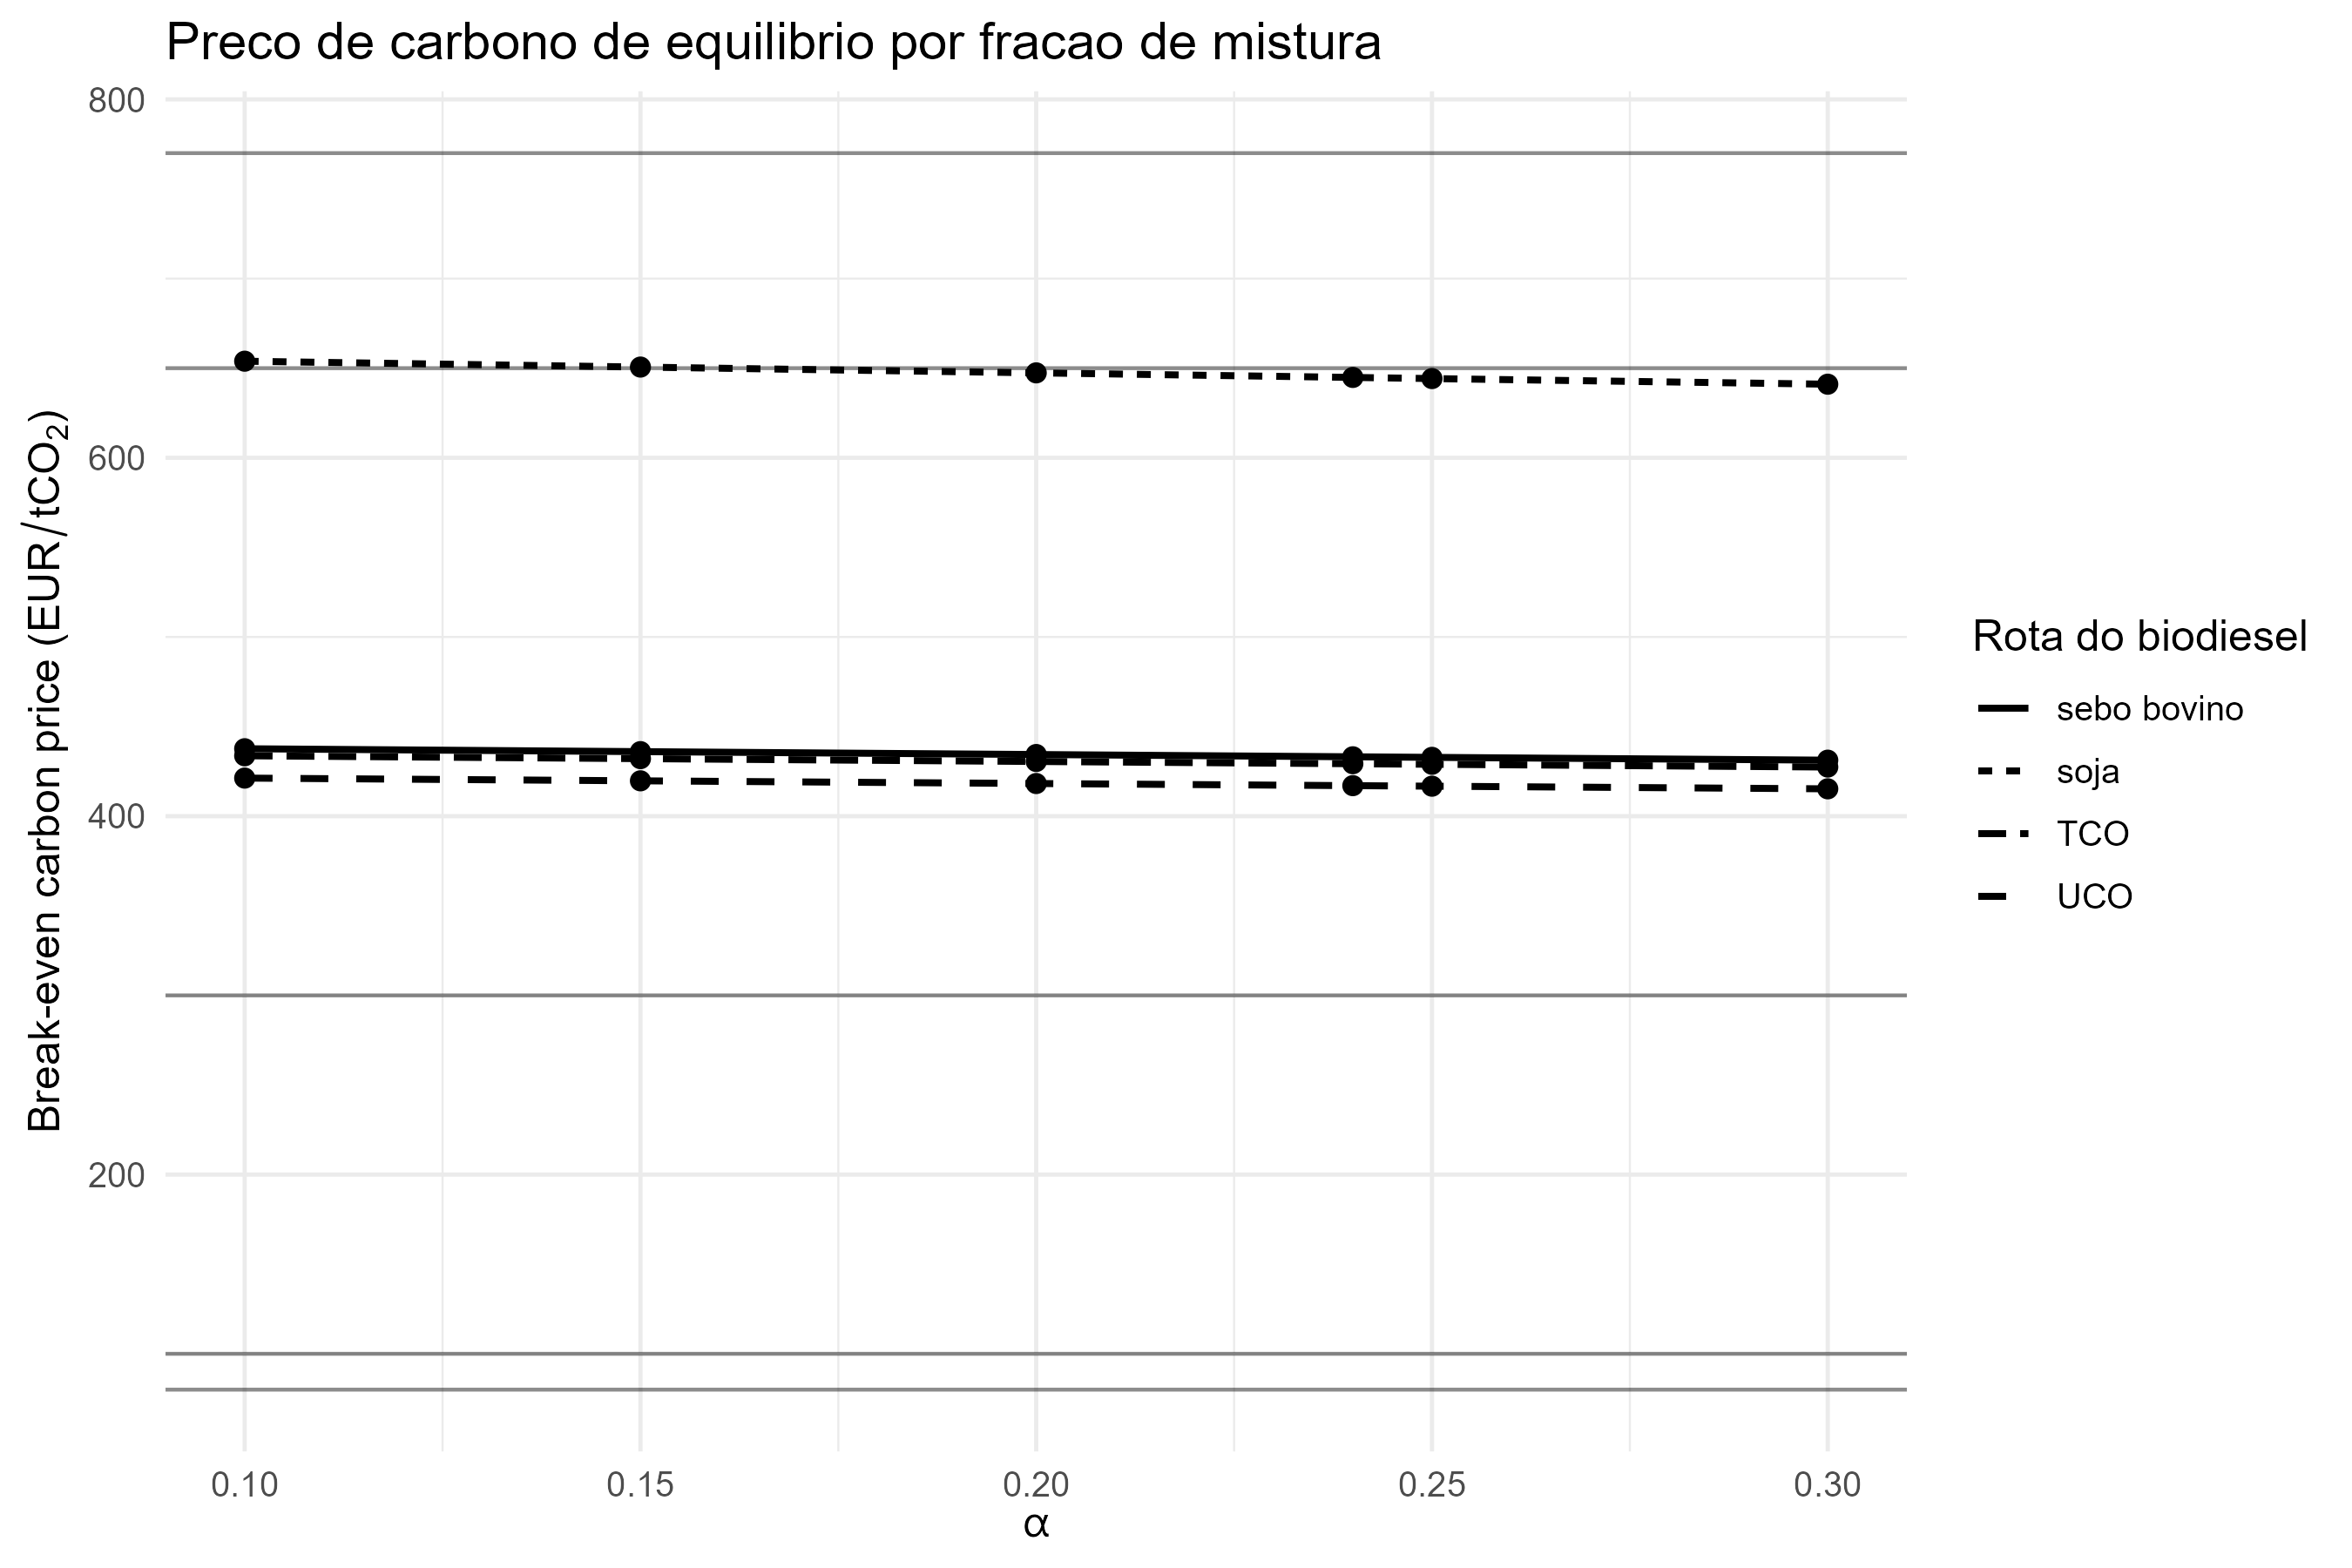
\includegraphics[width=0.85\textwidth]{grafico_03b_break_even_vs_alpha.png}
\caption{\warn{Preço de carbono de equilíbrio por fração de mistura e rota de biodiesel.}}
\label{fig:break_even_alpha}
\end{figure}

\warn{Os valores mínimos de preço de carbono de equilíbrio no cenário-base ocorrem em $\alpha = 0{,}30$ e são da ordem de $415,3\,\text{EUR}/tCO_2$ para \gls{UCO}, $427,4\,\text{EUR}/tCO_2$ para \gls{TCO}, $431,3\,\text{EUR}/tCO_2$ para sebo bovino e $641,1\,\text{EUR}/tCO_2$ para soja. Isso sugere que a atratividade relativa das rotas residuais ou de subprodutos industriais já se manifesta no modelo, mas ainda requer sinal regulatório mais forte do que o observado no mercado europeu de carbono, isto é, valores de $\gamma^{ref}$ significativamente superiores à faixa atualmente praticada no \gls{EUETS}.}

\warn{Em termos interpretativos, a Figura~\ref{fig:break_even_alpha} mostra mais do que uma simples ordenação entre rotas. Ela evidencia que o aumento de $\alpha$ melhora o desempenho relativo das alternativas renováveis no cenário-base, levando os menores preços de carbono de equilíbrio aos pontos de mistura mais altos testados. Isso indica que, na formulação atual, reduzir a fração renovável não é o caminho mais promissor para tornar o biobunker competitivo; ao contrário, as melhores condições econômicas relativas aparecem quando a mistura se aproxima do limite superior analisado.}

\begin{table}[!ht]
\centering
\caption{\warn{Preço de carbono de equilíbrio mínimo no cenário-base por rota de biodiesel}}
\label{tab:break_even_minimo}
\begin{tabular}{lccc}
\hline
\warn{Rota} & \warn{$\alpha$} & \warn{Break-even mínimo (EUR/tCO$_2$)} & \warn{Redução de emissões (\%)} \\
\hline
\warn{UCO} & \warn{0,30} & \warn{415,3} & \warn{21,6} \\
\warn{TCO} & \warn{0,30} & \warn{427,4} & \warn{21,5} \\
\warn{Sebo bovino} & \warn{0,30} & \warn{431,3} & \warn{20,8} \\
\warn{Soja} & \warn{0,30} & \warn{641,1} & \warn{14,0} \\
\hline
\end{tabular}
\end{table}

\warn{A Figura~\ref{fig:frontier_viabilidade} mostra a fronteira de viabilidade regulatória. Quando $\gamma^{ref}$ e $\gamma^{comp}$ são ampliados conjuntamente, os primeiros cenários viáveis aparecem a partir de aproximadamente $300\,\text{EUR}/tCO_2$, com destaque para \gls{UCO}, sebo bovino e \gls{TCO}. Para essas três rotas, as primeiras combinações viáveis ocorrem em torno de $\alpha = 0{,}24$, ao passo que a soja não se torna viável nem mesmo nos cenários regulatórios mais fortes testados.}

\warn{A utilidade desse gráfico está em transformar um resultado abstrato em fronteira observável de decisão. Em vez de afirmar apenas que determinados cenários ``não são viáveis'', a análise passa a mostrar em que patamar da família regulatória $\gamma$ a classificação muda. Isso permite interpretar a viabilidade como função conjunta de política climática, custo de \emph{compliance}, composição da mistura e, sobretudo, do nível de preço de carbono necessário para que o custo marginal de abatimento se torne compatível com o ambiente regulatório. No caso presente, a fronteira obtida indica que o \gls{EUETS} em níveis de mercado recentes é insuficiente, mas que regimes de indução mais fortes já colocam \gls{UCO}, sebo bovino e \gls{TCO} na região economicamente defensável.}

\begin{table}[!ht]
\centering
\caption{\warn{Primeiros cenários viáveis na exploração regulatória ampliada}}
\label{tab:primeiros_viaveis}
\begin{tabular}{lcccc}
\hline
\warn{Rota} & \warn{$\gamma^{ref}$ (EUR/tCO$_2$)} & \warn{$\gamma^{comp}$ (EUR/tCO$_2$)} & \warn{$\alpha$} & \warn{Redução (\%)} \\
\hline
\warn{UCO} & \warn{300} & \warn{300} & \warn{0,24} & \warn{17,1} \\
\warn{TCO} & \warn{300} & \warn{300} & \warn{0,24} & \warn{17,0} \\
\warn{Sebo bovino} & \warn{300} & \warn{300} & \warn{0,24} & \warn{16,5} \\
\warn{Soja} & \warn{--} & \warn{--} & \warn{--} & \warn{--} \\
\hline
\end{tabular}
\end{table}

\begin{figure}[!ht]
\centering
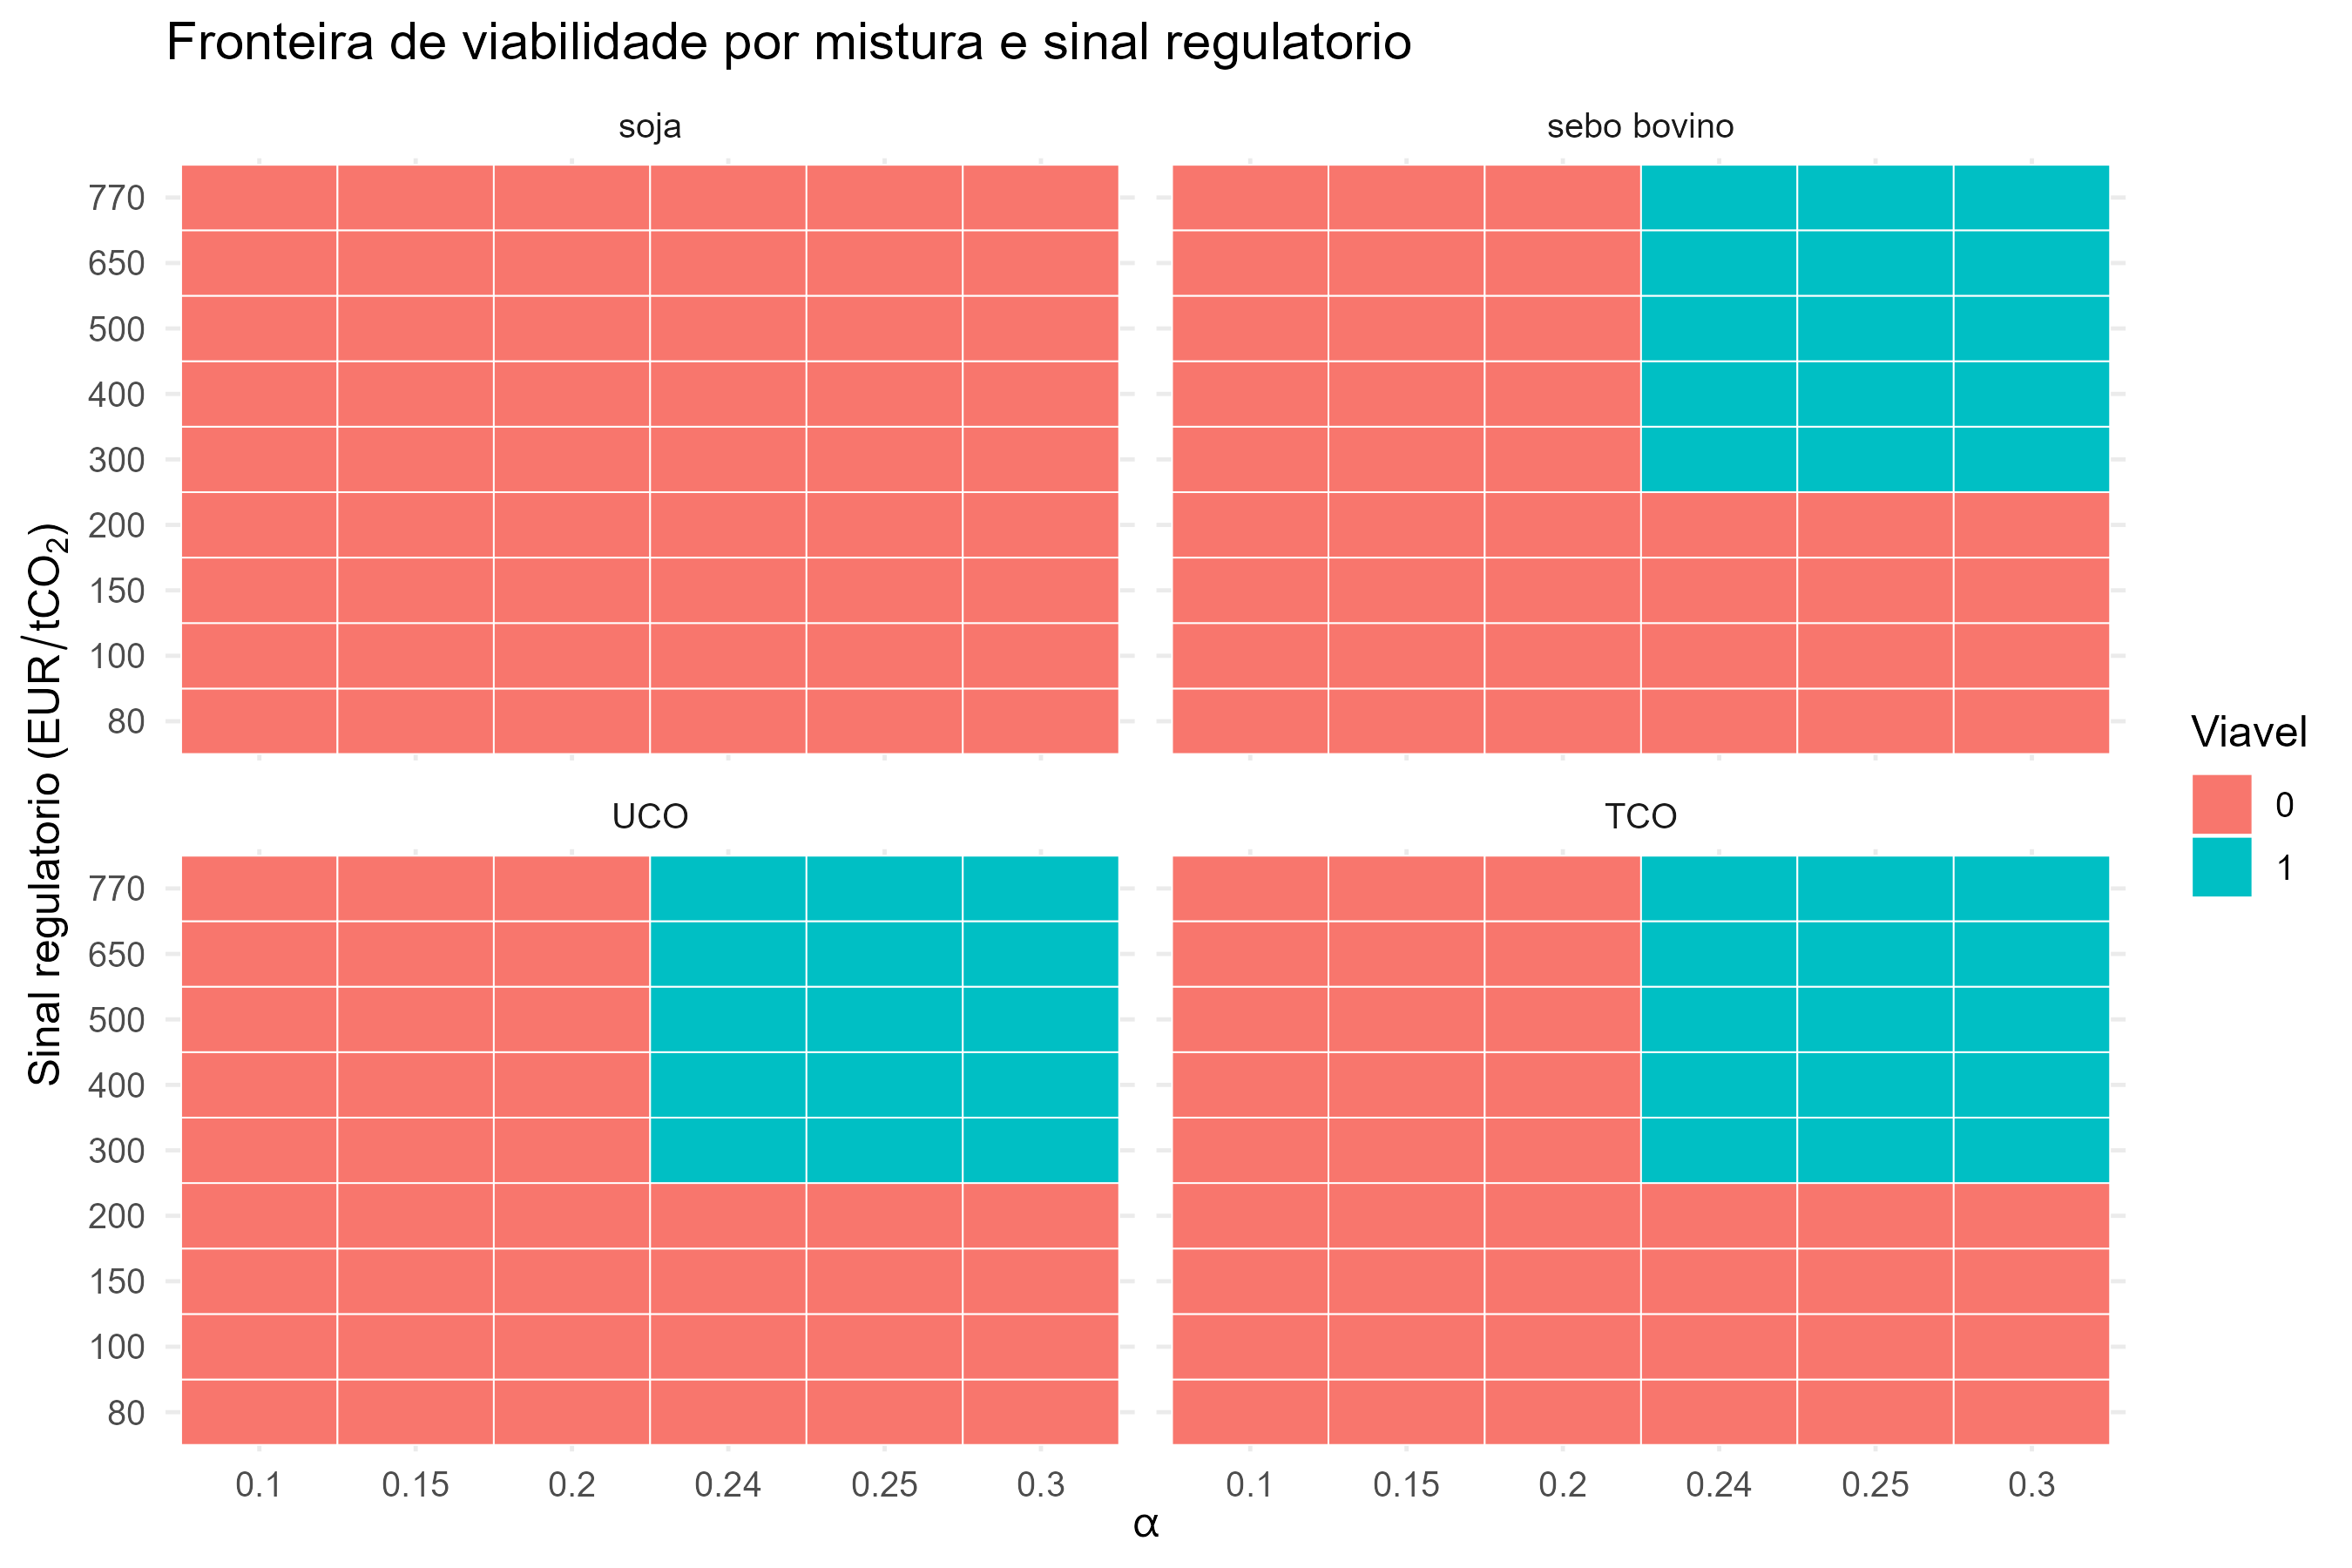
\includegraphics[width=0.95\textwidth]{grafico_07_fronteira_viabilidade.png}
\caption{\warn{Fronteira de viabilidade econômico-ambiental por fração de mistura, rota e sinal regulatório ampliado.}}
\label{fig:frontier_viabilidade}
\end{figure}

\warn{A leitura de custo também se altera quando o termo regulatório é explicitado. A Figura~\ref{fig:decomp_custo} decompõe o custo total entre combustível e a parcela de \emph{compliance} associada a $\gamma^{comp}$. Essa visualização evidencia que o custo regulatório cresce com a parcela fóssil remanescente, mas ainda não compensa, por si só, o diferencial de preço do biodiesel nos níveis correntes de mercado. Em outras palavras, o \gls{EUETS} melhora a competitividade relativa do biobunker, mas não basta sozinho para torná-lo viável sob os parâmetros-base.}

\warn{Esse ponto é importante porque evita uma leitura simplificada do papel da regulação. O componente $\gamma^{comp}$ atua como mecanismo de mitigação do diferencial econômico entre fóssil e biobunker, mas não elimina esse diferencial no nível atual de preços adotado na simulação. Assim, a análise preliminar sugere que a viabilidade depende menos de relaxar o critério ambiental e mais de combinar três alavancas: maior $\gamma^{ref}$, maior $\gamma^{comp}$, redução do preço relativo do biodiesel e escolha de rotas com menor intensidade de carbono, como \gls{UCO}, sebo bovino e \gls{TCO}.}

\begin{figure}[!ht]
\centering
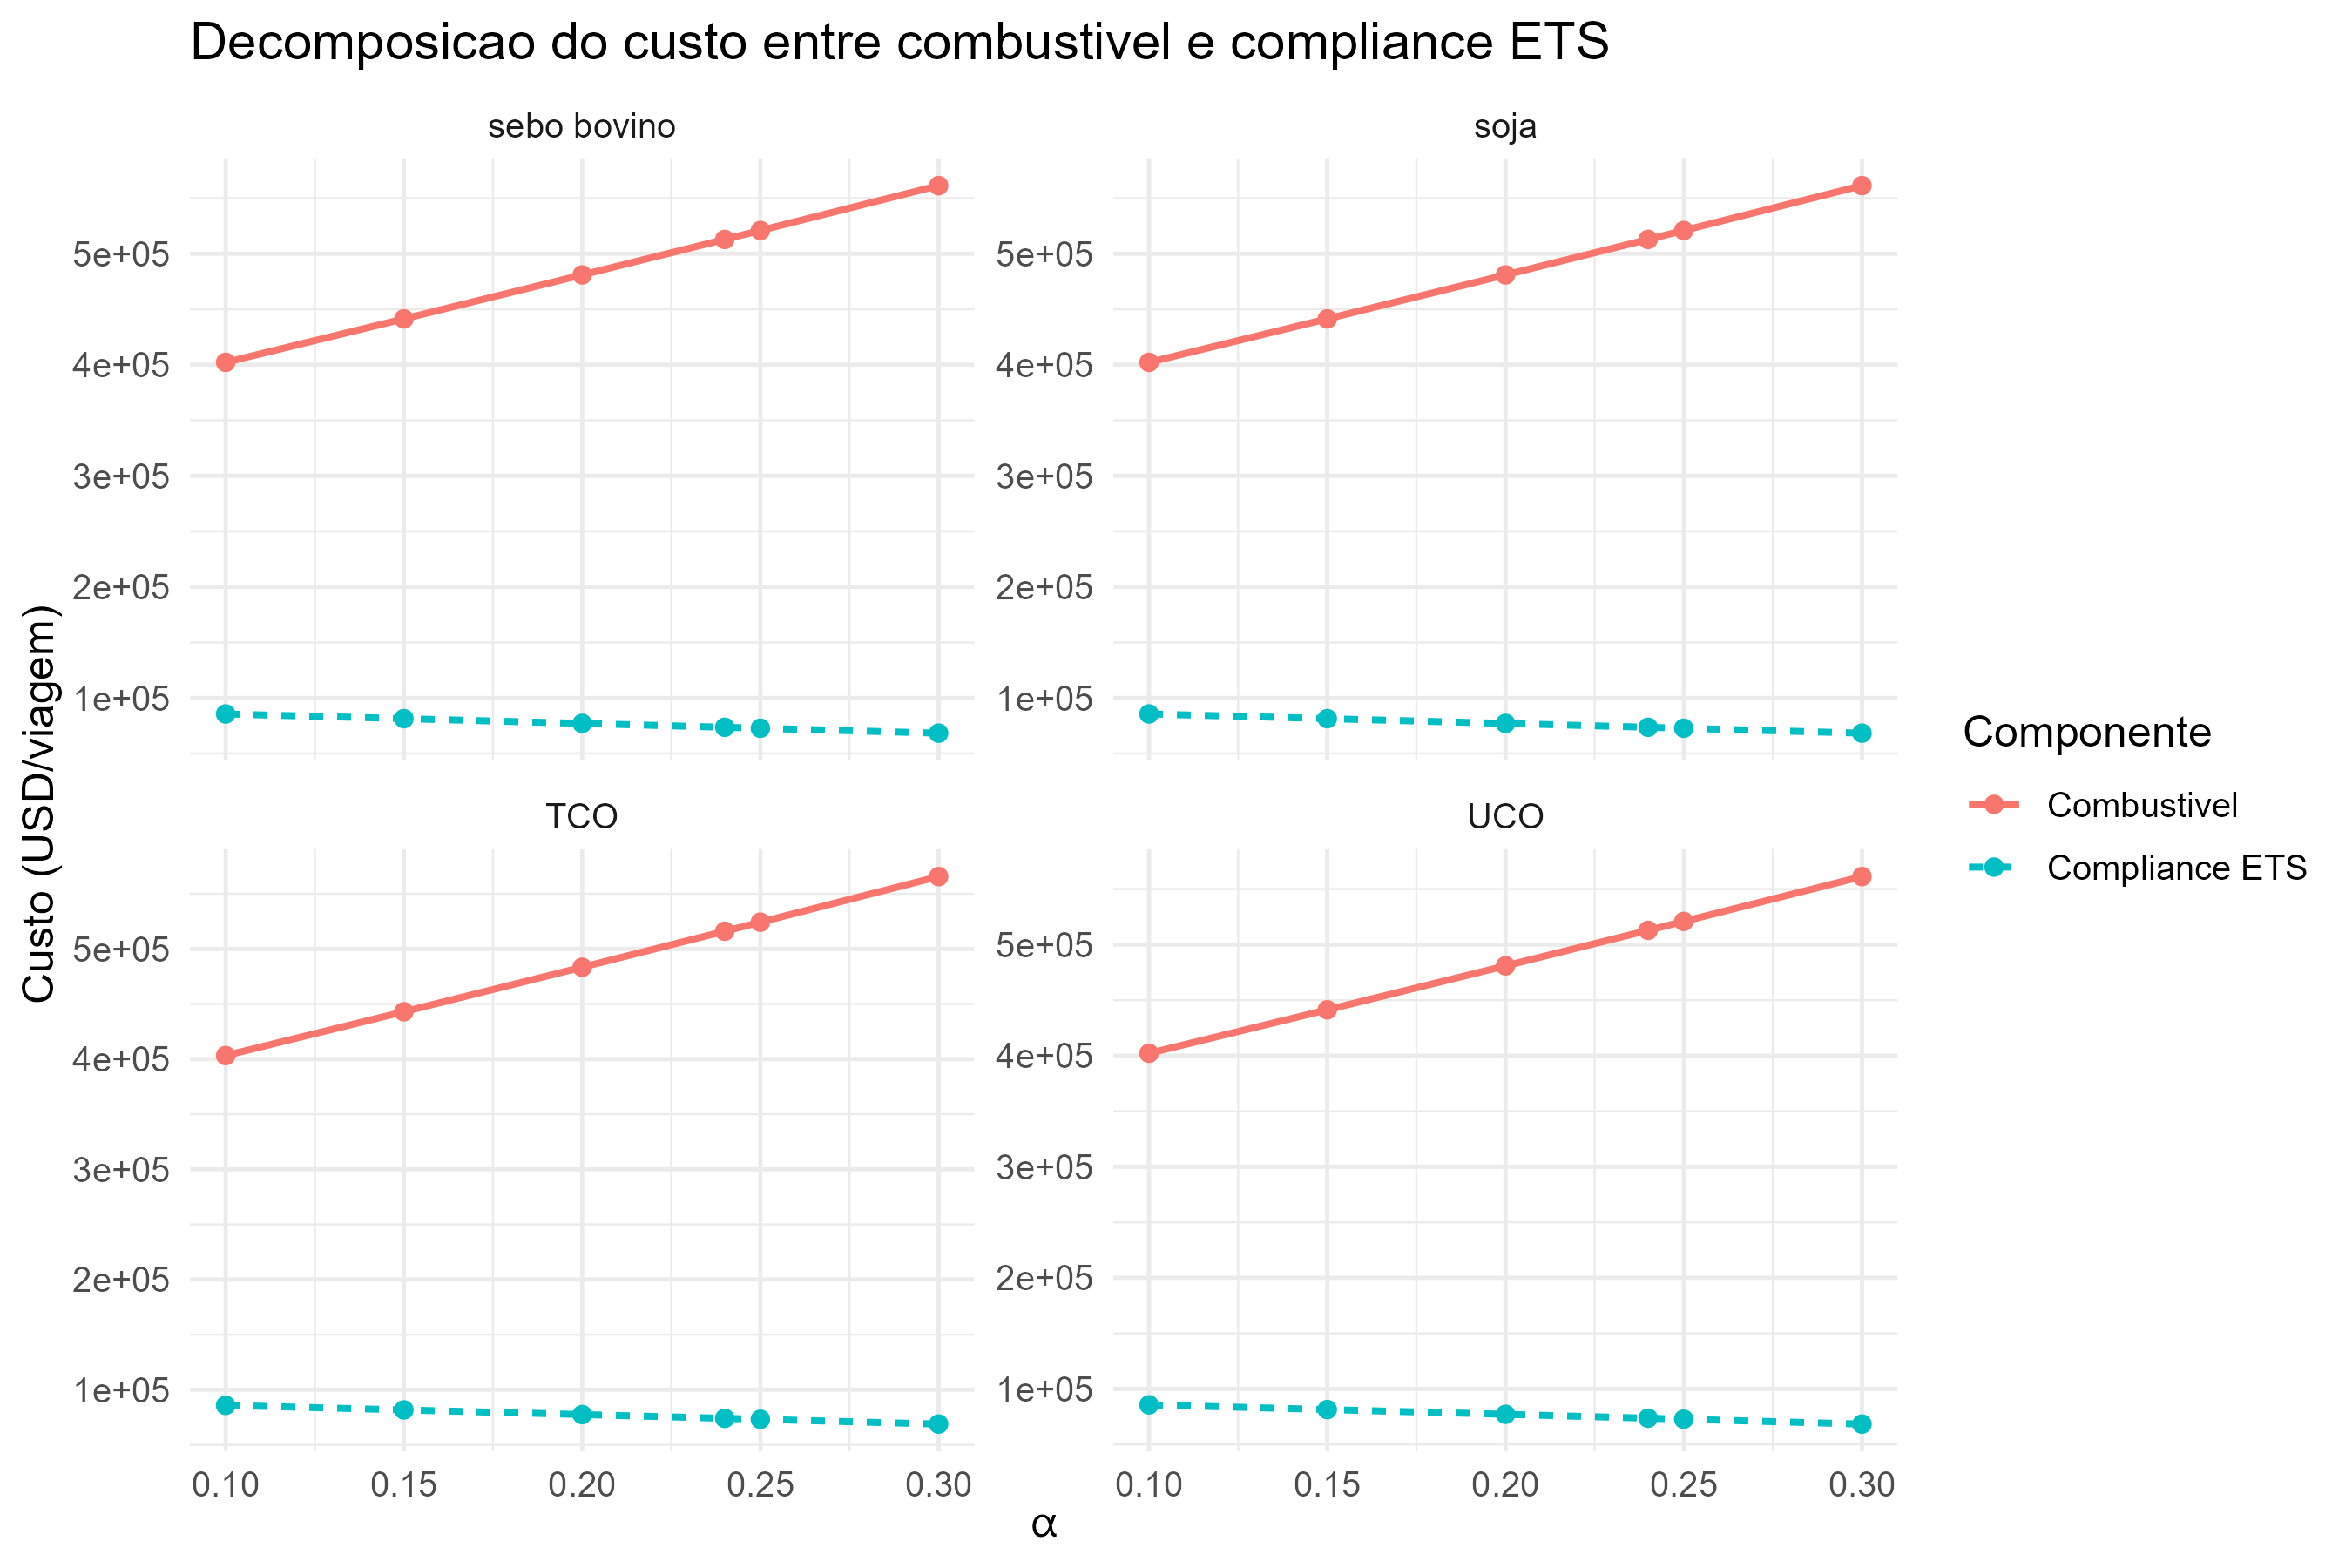
\includegraphics[width=0.95\textwidth]{grafico_06_decomposicao_custo.png}
\caption{\warn{Decomposição do custo total entre custo de combustível e custo de \emph{compliance} do \gls{EUETS}.}}
\label{fig:decomp_custo}
\end{figure}

\warn{No caso específico de \gls{TCO}, a análise preliminar indica desempenho próximo ao de \gls{UCO} e sebo bovino quando se utilizam os parâmetros-base. Entretanto, a sensibilidade específica dessa rota mostra que sua atratividade depende de forma relevante do fator de emissão \gls{WTW} e, sobretudo, do preço relativo do biodiesel produzido a partir desse subproduto. Essa evidência reforça a necessidade de tratar \gls{TCO} como rota promissora, porém mais sensível a escolhas metodológicas e econômicas do que as rotas residuais mais consolidadas.}

\warn{Em síntese, os resultados preliminares apontam três conclusões centrais}. \warn{Primeiro, o custo marginal de abatimento dos cenários avaliados permanece acima do intervalo de referência $\gamma^{ref}$ sob condições atuais, caracterizando inviabilidade econômica-regulatória.} \warn{Primeiro, a inviabilidade do biobunker sob sinal regulatório de carbono na faixa recente do \gls{EUETS}. Segundo, a emergência de cenários viáveis para \gls{UCO}, sebo bovino e \gls{TCO} quando se simulam regimes de indução regulatória mais fortes. Terceiro, a utilidade analítica do preço de carbono de equilíbrio como métrica-síntese para comparar rotas, frações de mistura e condições regulatórias em um mesmo quadro interpretativo.}


\chapter{Considerações parciais}
\label{chap_conclusao}

Esta dissertação, em sua versão de qualificação, investigou se, sob premissas técnicas de compatibilidade operacional, o biobunker pode ser considerado alternativa econômico-ambientalmente viável para apoiar a transição energética do transporte marítimo internacional operando a partir do Brasil, considerando as metas intermediárias de descarbonização da \gls{IMO} até 2030 e os condicionantes regulatórios associados a rotas internacionais. Para responder a essa questão, o trabalho desenvolveu modelo determinístico de simulação comparativa aplicado à rota Santos--Roterdã, articulando condições operacionais representativas, fatores de emissão em escopo \emph{well-to-wake}, custos de combustível, custo explícito de \emph{compliance} do \gls{EUETS} e critério de viabilidade baseado no custo marginal de abatimento de carbono.

À luz do critério de viabilidade adotado no modelo, a resposta à pergunta de pesquisa é negativa no cenário-base e positiva apenas de forma condicional em cenários regulatórios ampliados. No cenário-base e sob sinal regulatório compatível com a faixa recente do \gls{EUETS}, o biobunker não se mostra econômico-ambientalmente viável para nenhuma das rotas de produção avaliadas. Em todos os cenários simulados, o custo marginal de abatimento permanece acima do intervalo de referência adotado para o ambiente europeu de precificação de carbono. Isso significa que, embora a substituição parcial do combustível fóssil produza reduções de emissões, o ganho ambiental obtido não é suficiente, nas condições-base do modelo, para compensar o diferencial de custo da mistura frente ao patamar regulatório atualmente observado. Essa conclusão vale no escopo determinístico e paramétrico da modelagem, aplicado à rota Santos--Roterdã e sob os parâmetros médios adotados.

Ao mesmo tempo, os resultados mostram que essa resposta não deve ser interpretada de forma absoluta. A análise comparativa entre rotas de produção do biodiesel evidencia heterogeneidade relevante entre matérias-primas. Rotas associadas a \gls{UCO}, sebo bovino e \gls{TCO} apresentam desempenho superior ao da soja tanto em termos ambientais quanto em termos de preço de carbono de equilíbrio. Além disso, quando se ampliam conjuntamente os parâmetros regulatórios do modelo, passam a emergir cenários viáveis para \gls{UCO}, sebo bovino e \gls{TCO}, particularmente a partir de misturas em torno de \gls{B24}. Nesse sentido, os resultados parciais sustentam que o biobunker não é alternativa econômico-ambientalmente viável sob condições regulatórias correntes, mas passa a se mostrar econômico-ambientalmente viável nos cenários regulatórios ampliados simulados quando associado a matérias-primas de menor intensidade de carbono.

Esses achados permitem apresentar, já na qualificação, três contribuições principais do trabalho. A primeira consiste na proposição de um arcabouço analítico integrado capaz de avaliar, em um mesmo modelo, a articulação entre demanda útil constante, emissões \emph{WTW}, custo total por viagem e custo marginal de abatimento de carbono, evitando leituras isoladas apenas ambientais ou apenas econômicas. A segunda consiste na aplicação desse arcabouço a um caso representativo do transporte marítimo internacional operando a partir do Brasil, incorporando explicitamente a heterogeneidade entre rotas de produção do biodiesel e mostrando como diferenças de matéria-prima alteram o espaço de viabilidade. A terceira consiste na articulação entre modelagem quantitativa e interpretação regulatória, por meio da distinção entre custo explícito de \emph{compliance} e parâmetro de referência para avaliação da atratividade econômico-ambiental, o que permite ler a viabilidade do biobunker como resultado conjunto de custo, emissões e indução regulatória.

Como se trata ainda de etapa de qualificação, estas considerações têm caráter parcial e devem ser entendidas como base para aprofundamento posterior da dissertação. O estudo já permite delimitar com clareza o comportamento do modelo, as diferenças entre rotas e o papel do ambiente regulatório, mas também evidencia frentes concretas de continuidade metodológica e empírica. Entre elas, destacam-se o refinamento do domínio de mistura, o desacoplamento entre os sinais regulatórios do modelo, a expansão para novas rotas marítimas e o desenvolvimento de versões mais sensíveis à incerteza dos parâmetros econômicos, ambientais e operacionais.

Além dessas extensões de modelagem, a etapa seguinte do trabalho deverá priorizar a calibração empírica mais fina das rotas de biodiesel a partir de informações associadas ao contexto produtivo brasileiro. Isso envolve, por exemplo, o levantamento de dados mais precisos sobre preços, capacidade de oferta, distribuição regional de produção, matérias-primas predominantes e condições logísticas de abastecimento, com base em informações públicas de empresas brasileiras produtoras de biodiesel, associações setoriais, relatórios institucionais e bases regulatórias. Esse aprofundamento é relevante porque permitirá reduzir a dependência de parâmetros médios mais agregados e aproximar o modelo de condições mais realistas de formação de custo e disponibilidade das rotas analisadas.

No mesmo sentido, a continuidade da pesquisa deverá combinar ajustes no arquivo \texttt{simulacao.R} com nova rodada de análise dos resultados. Espera-se, nessa etapa, revisar a parametrização-base, atualizar sinais regulatórios e preços de referência, incorporar informações mais precisas sobre as rotas associadas a soja, sebo bovino, \gls{UCO} e \gls{TCO}, e avaliar se essas revisões alteram a fronteira de viabilidade identificada nesta versão. Paralelamente, a maturação do trabalho exigirá a consolidação desses achados em forma de artigo e o adensamento da redação final da dissertação, de modo a transformar os resultados parciais aqui apresentados em versão final consistente para defesa.

Com base nesse encaminhamento, a Tabela~\ref{tab:cronograma_qualificacao_defesa} apresenta o cronograma estratégico previsto do período posterior à qualificação até a defesa, tomando como referência o início das atividades em maio e o encerramento em dezembro.

\begin{table}[!ht]
\centering
\caption{Cronograma estratégico da qualificação à defesa}
\label{tab:cronograma_qualificacao_defesa}
\scriptsize{
\begin{tabular}{l c c c c c c c c}
\toprule
\multirow{2}{*}{Atividade} & \multicolumn{8}{c}{Meses} \\
& mai & jun & jul & ago & set & out & nov & dez \\
\midrule
Implementação & X & X & X & & & & & \\
Análise & & X & X & X & X & & & \\
Escrita de artigo & & & & X & X & X & & \\
Escrita da dissertação & & & X & X & X & X & X & \\
Defesa & & & & & & & & X \\
\bottomrule
\end{tabular}
}
\end{table}

Em termos estratégicos, a fase de implementação concentra os ajustes no modelo e na base empírica, incluindo a incorporação de parâmetros mais realistas para as rotas de biodiesel e eventuais modificações necessárias no \texttt{simulacao.R}. A fase de análise cobre a reexecução dos experimentos, a comparação entre resultados atualizados e os resultados parciais desta qualificação, bem como a interpretação das mudanças na fronteira de viabilidade. A escrita de artigo funciona como esforço de síntese e amadurecimento dos resultados centrais, enquanto a escrita da dissertação acompanha e consolida todo o processo até a preparação final para defesa.

Em síntese, esta etapa de qualificação já permite afirmar que o biobunker não se revela econômico-ambientalmente viável sob o ambiente regulatório corrente representado no cenário-base, mas tampouco deve ser tratado como alternativa irrelevante. Quando avaliado sob critérios explícitos de desempenho ambiental, custo e regulação, ele se apresenta como rota de transição condicional, cuja relevância depende da combinação concreta entre matéria-prima, mistura, contexto operacional e intensidade da indução regulatória. A etapa seguinte do trabalho deverá justamente aprofundar essa conclusão parcial, ampliando a base empírica do modelo e refinando os parâmetros que aproximam a simulação das condições efetivas do setor brasileiro de biodiesel e do transporte marítimo internacional.


\appendix

\chapter{Glossário de termos metodológicos}
\label{ap:glossario_metodologico}

Este apêndice reúne definições curtas de termos metodológicos e analíticos recorrentes na dissertação. O objetivo é oferecer apoio de leitura a públicos não especializados em modelagem, simulação e análise quantitativa, preservando no texto principal a fluidez da argumentação.

\begin{description}
    \item[Algoritmo] Sequência ordenada de etapas usada para executar um cálculo, resolver um problema ou gerar resultados a partir de dados de entrada.

    \item[Analítico] Relativo à decomposição de um problema em partes e relações formais, de modo a permitir interpretação estruturada dos resultados.

    \item[Cenário] Combinação específica de hipóteses, parâmetros e condições de análise usada para representar uma situação possível no modelo.

    \item[Cenário-base] Cenário de referência a partir do qual os demais cenários são comparados. Nesta dissertação, ele corresponde ao uso do \emph{bunker fuel} convencional nas condições operacionais da rota analisada.

    \item[Critério de viabilidade] Regra adotada para classificar um cenário como viável ou não. No presente estudo, esse critério combina simultaneamente um requisito mínimo de redução de emissões e um requisito econômico-regulatório.

    \item[Custo marginal de abatimento] Indicador que relaciona o custo adicional de uma alternativa à quantidade de emissões que ela evita. Ele mostra quanto custa reduzir uma tonelada adicional de dióxido de carbono equivalente.

    \item[Determinístico] Tipo de modelagem em que os resultados decorrem diretamente dos valores de entrada definidos, sem incorporar sorteios aleatórios ou distribuições probabilísticas.

    \item[Domínio do modelo] Conjunto de combinações admissíveis entre variáveis e parâmetros que o modelo efetivamente examina.

    \item[Hipótese operacional] Formulação testável, expressa nos termos do próprio modelo, que orienta a verificação principal do estudo.

    \item[Modelo de simulação] Representação simplificada de um sistema real usada para calcular o comportamento esperado desse sistema sob diferentes condições.

    \item[Parâmetro] Quantidade tratada como dada no modelo, usada para caracterizar condições de operação, preços, fatores de emissão ou demais propriedades relevantes.

    \item[Robustez] Grau em que um resultado se mantém estável quando certas hipóteses ou parâmetros do modelo são alterados.

    \item[Sensibilidade] Medida de quanto os resultados do modelo mudam quando uma ou mais entradas são alteradas.

    \item[Simulação] Procedimento de execução do modelo para reproduzir, de forma simplificada, o comportamento de um sistema em condições específicas.

    \item[Estocástico] Tipo de modelagem que incorpora incerteza explicitamente, representando variáveis por distribuições probabilísticas ou mecanismos aleatórios.

    \item[Variável] Grandeza cujo valor pode mudar entre cenários ou ao longo da modelagem, influenciando ou representando os resultados do sistema analisado.

    \item[Varredura paramétrica] Procedimento em que um ou mais parâmetros são alterados sistematicamente dentro de um intervalo predefinido para observar como os resultados respondem a essas mudanças.
\end{description}

\chapter{Planejamento experimental complementar}
\label{ap:planejamento_experimental}

Este apêndice registra extensões de análise que podem fortalecer a dissertação em etapas posteriores, mas que exigem nova execução do arquivo \texttt{simulacao.R} ou alteração do próprio script. O objetivo, nesta fase de qualificação, é separar com clareza o que já foi incorporado ao texto com base nos resultados existentes daquilo que demandaria esforço computacional ou modelagem adicional.

\section{Experimentos que exigem nova execução com a estrutura atual do script}

O arquivo \texttt{simulacao.R} já implementa sete \emph{setups} principais e pode ser reexecutado, sem alteração estrutural, para atualizar resultados quando houver necessidade de revisar premissas paramétricas. Entre os casos mais imediatos, destacam-se os seguintes:

\begin{enumerate}
    \item atualização dos parâmetros econômicos de referência, como preço do \emph{bunker fuel}, preço do biodiesel por rota e taxa de câmbio EUR/USD, para refletir nova janela temporal de mercado;
    \item atualização do sinal regulatório europeu, sobretudo dos valores de $\gamma^{ref}$ e $\gamma^{comp}$, caso se deseje aproximar o modelo de nova faixa observada no \gls{EUETS};
    \item atualização dos fatores de emissão \gls{WTW} das rotas de biodiesel, caso novas estimativas bibliográficas sejam adotadas para \gls{UCO}, sebo bovino, soja ou \gls{TCO};
    \item reexecução dos gráficos e tabelas de sensibilidade econômica, ambiental, regulatória, operacional e específica de \gls{TCO}, a partir de qualquer revisão dos parâmetros-base já definidos no script.
\end{enumerate}

\section{Experimentos que exigem alteração do \texttt{simulacao.R}}

Algumas extensões relevantes para uma etapa posterior do trabalho já podem ser delineadas, mas demandam modificação explícita do código atual.

\subsection{Desacoplamento entre os sinais regulatórios}

No \emph{Setup} E6, a trajetória regulatória ampliada é implementada com aumento simultâneo de $\gamma^{ref}$ e $\gamma^{comp}$. Uma extensão metodologicamente útil consiste em desacoplar esses dois componentes, permitindo testar cenários em que o preço de referência do carbono e o custo efetivo de \emph{compliance} evoluem em velocidades diferentes. Isso exigiria:

\begin{enumerate}
    \item redefinir a tabela \texttt{policy\_tbl} com combinações independentes entre os dois sinais;
    \item reexecutar o cálculo dos cenários E6;
    \item gerar novas figuras de fronteira regulatória e novas tabelas-resumo.
\end{enumerate}

\subsection{Refinamento do domínio de mistura}

O modelo atual avalia $\alpha$ em um conjunto discreto de valores. Caso se deseje investigar com maior precisão a transição entre inviabilidade e viabilidade, especialmente no intervalo entre $\alpha=0{,}24$ e $\alpha=0{,}30$, será necessário:

\begin{enumerate}
    \item redefinir o vetor \texttt{alpha\_grid} com malha mais fina;
    \item reexecutar os \emph{setups} E1, E4 e E6;
    \item regenerar os gráficos de preço de carbono de equilíbrio, fronteira regulatória e \emph{trade-off}.
\end{enumerate}

\subsection{Expansão para múltiplas rotas marítimas}

O script atual está parametrizado com foco na rota Santos--Roterdã. A inclusão de outras rotas exigiria alteração do código para leitura ou definição de novos vetores operacionais $(D,V,c)$, bem como a organização de uma camada adicional de comparação entre trajetos. Esse passo é particularmente relevante para estudos posteriores voltados à robustez externa dos resultados.

\subsection{Modelagem estocástica}

O modelo implementado é determinístico e paramétrico. Uma extensão natural consiste em introduzir incerteza explícita, por exemplo por simulação de Monte Carlo para preços, fatores de emissão, parâmetros operacionais e câmbio. Essa ampliação exigiria:

\begin{enumerate}
    \item definição de distribuições probabilísticas para os parâmetros de entrada;
    \item criação de nova rotina de simulação no \texttt{simulacao.R};
    \item redefinição das saídas para incluir intervalos, distribuições e probabilidades de viabilidade.
\end{enumerate}

\subsection{Custos adicionais de adaptação e logística}

O modelo atual representa a viagem a partir de custo de combustível e custo de \emph{compliance} regulatório. Em uma fase posterior, pode ser útil adicionar custos associados a armazenagem, \emph{bunkering}, segregação, adaptação operacional ou logística portuária. Essa extensão exigiria novas equações de custo e nova parametrização empírica, além de rerun completo dos experimentos centrais.

\section{Uso recomendado deste planejamento}

Para a fase de qualificação, o texto principal da dissertação deve priorizar os resultados já efetivamente gerados e discutidos. As extensões registradas neste apêndice funcionam como agenda metodológica explícita para aprofundamento posterior, sem confundir o leitor quanto ao que já foi executado e ao que ainda depende de nova rodada computacional ou de modificação do modelo.


\newcommand{\Extrachap}[1]{\chapter*{#1}\markboth{#1}{#1}%
\addcontentsline{toc}{chapter}{#1}}

\Extrachap{Referências}

\renewcommand{\bibsection}{}
\renewcommand{\bibname}{}
\bibliography{references}

\label{lastpage}
\end{document}
